\chapter{Flujo de trabajo y Aplicación Web}

\begin{figure}[H]
    \centering
    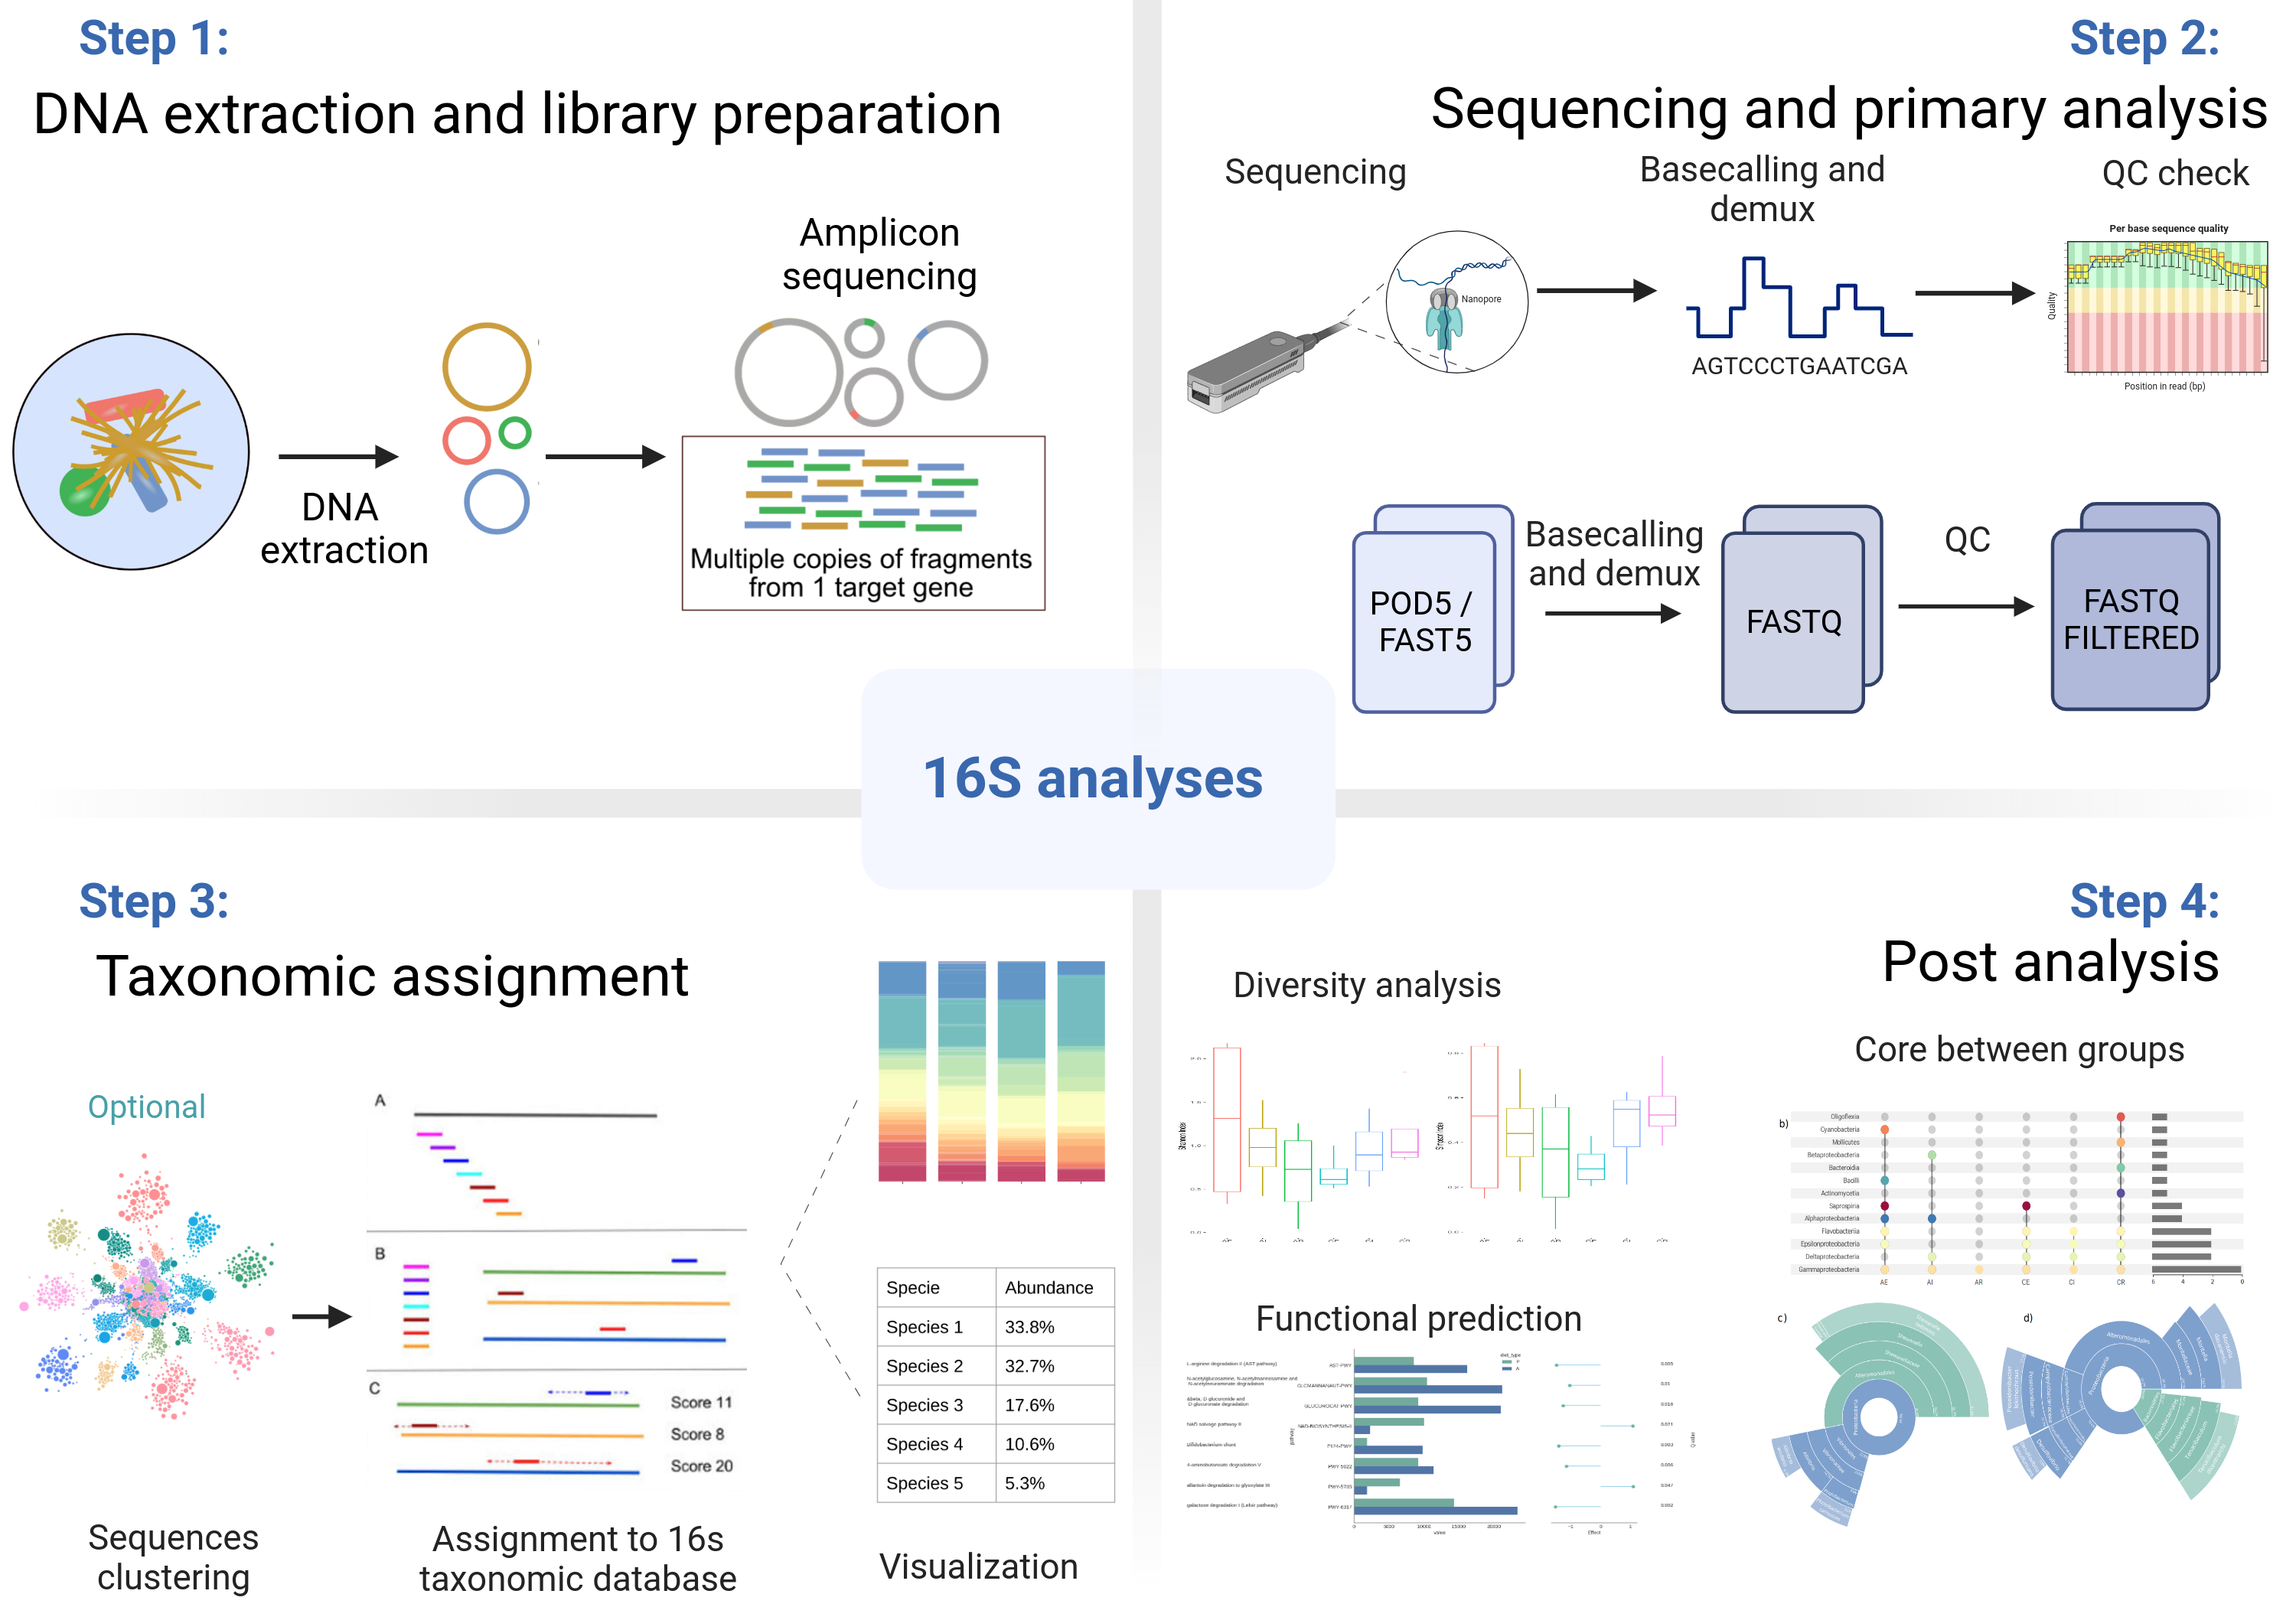
\includegraphics[width=1\linewidth]{images/16s_workflow_schema.jpeg}
    \caption{Flujo de trabajo estándar para la secuenciación y análisis de secuenciaciones del gen 16S}
    \label{fig:16S_workflow}
\end{figure}
\section{Flujo de trabajo}
Se desarrolló un flujo de trabajo automatizado en Nextflow que permite el análisis y la caracterización de secuencias del gen 16S obtenidas mediante dispositivos de secuenciación de Oxford Nanopore. 
El pipeline cuenta con los siguientes módulos: Basecalling y demultiplexación (\textit{basecalling}), Control de calidad (\textit{qc}), Asignación taxonómica (\textit{taxonomic\_assignament}), Indices de diversidad (\textit{diversity}) y Predicción funcional (\textit{functional\_predicction}).

El flujo de trabajo está diseñado de manera modular permitiendo que el usuario pueda personalizar su ejecución, agregando o quitando módulos de análisis mediante un archivo de configuración. 

\subsection{Archivo de configuración}
Este archivo permite activar o desactivar cada módulo de manera individual y especificar parámetros para modificar su ejecución. 
Además, el archivo de configuración incluye información sobre los archivos de entrada del flujo de trabajo, nombres de las muestras y grupos asociados, todo en un formato de diccionario.

Para ejecutar el flujo de trabajo se requiere un archivo de configuración en formato YAML que contenga los parámetros necesarios para la ejecución del pipeline. 
A continuación se presenta un ejemplo de archivo de configuración:



\subsection{Estructura del flujo de trabajo}
\subsubsection{Basecalling y demultiplexación}
\hl{hacer}
\subsubsection{Control de calidad}
Este módulo siempre se ejecuta  \hl{excepto que..} y es el encargado de realizar los filtros y control de calidad de las muestras.
La entrada de este módulo son archivos en formato \textit{Fastq}, que pueden ser provenientes del módulo anterior (\textit{basecalling y demultiplexación}) o pueden ser indicados por el usuario a través del archivo de configuración.
El control de calidad se realiza mediante la herramienta NanoPlot (antes y después de los filtros).
Los filtros de calidad son llevados a cabo con la herramienta Fastp, utilizando los siguientes parámetros:
\begin{itemize}
    \item calidad mínima: por defecto 10 o valor ingresado en el archivo de configuración qc.min\_qscore (\textit{-q 10})
    \item \textit{--cut\_front} 
    \item \textit{--cut\_tail} 
    \item \textit{--cut\_mean\_quality 10} 
    \item longitud mínima requerida: por defecto 1000 o valor ingresado en el archivo de configuración qc.min\_length (\textit{--length\_required 1000}) 
    \item longitud máxima permitida: por defecto 2000 o valor ingresado en el archivo de configuración qc.max\_length (\textit{--length\_limit 2000})
    \item deshabilitar la eliminación de adaptadores (\textit{--disable\_adapter\_trimming}) (no modificable)
    \item deshabilitar la eliminación de colas poly g (\textit{--disable\_trim\_poly\_g}) (no modificable)
\end{itemize}

A demás, este módulo cuenta con un script desarrollado en Python que permite graficar la longitud promedio versus la calidad promedio de las muestras después de los filtros \hl{se demora mucho y lo comente, descomentar y ver que onda el plot}.

El output de este módulo es una carpeta llamada \textit{QC} que contiene los siguientes directorios:
\begin{itemize}
    \item \textit{fastq\_filtered}: Directorio con archivos FASTQ de las secuencias filtradas (obtenidos con fastp).
    \item \textit{fastp\_reports}: Directorio con los reportes de los filtros de calidad en formato JSON y HTML (obtenidos con fastp).
    \item \textit{nanoplot\_reports}: Directorio con los reportes de control de calidad de las muestras antes y después de los filtros (obtenidos con NanoPlot).
    \item \hl{multiqc}
    \item \hl{quality plot}
\end{itemize}

\subsubsection{Asignación taxonómica}
Este módulo se ejecuta siempre que el parámetro de asignación taxonómica sea ``ON'' en el archivo de configuración.\hl{deberia ser siempre no xD}.
La entrada de este módulo son archivos en formato \textit{FASTQ} que provienen del módulo anterior (\textit{control de calidad}).

Previo a la asignación taxonómica, se realiza un subsampleo de las muestras con la herramienta Seqkit para evitar sesgos en la caracterización de la comunidad microbiana debido a alguna desproporción en la cantidad de lecturas de las muestra.
La cantidad de lecturas utilizadas para el subsampling por defecto es 100.000 o el valor ingresado por el usuario en el archivo de configuración \textit{qc.subsampling}.
Posterior a ello se convierten los archivos FASTQ a formato FASTA mediante la herramienta Seqkit.

La asignación taxonómica se realiza mediante la herramienta BLAST con la base de datos de 16S de Genbank.\hl{parámetros}

Posterior a la asignación taxonómica, mediante la herramienta TaxonKit se obtiene el linaje completo de todas las especies asignadas con Blast, este resultado se formatea mediante la herramienta CSVTk. 
Esto se realiza con el objetivo de poder graficar todas las categorías taxonómicas tanto en los gráficos de barras apilas como en el gráfico circular jerárquico.

Mediante un script en python se realiza un resumen de la asignación taxonómica obtenida con BLAST de todas las muestras y los linajes asociados a cada especie en un solo archivo. Además, se generan archivos por cantidad de lecturas y porcentaje, por cada categoría taxonómica y por muestra y grupo (en caso de ingresarse).
Estos archivos son utilizandos como entradas para los scripts que generan los gráficos de barras apiladas y  el gráfico circular jerárquico.


En el caso del gráfico circular, se buscan todas las taxonomías compartidas entre las muestras que tengan una abundance mayor al 1\% en al menos una muestra. 
Una vez que se identifican, se suman las lecturas asignadas a cada taxonomía en todas las muestra del grupo y se grafica el porcentaje de lecturas asignadas a cada taxonomía en todas las muestras del grupo como un valor único.

El output de este módulo es una carpeta llamada \textit{taxonomic\_assignament} que contiene los siguientes directorios:
\begin{itemize}
\item blast\_out
\item plots: Este directorio contiene los siguientes directorios:
\begin{itemize}
    \item taxonomy\_plots: Directorio con los gráficos de barras apiladas de las taxonomías. Contiene cuatro tipos de graficos: 
    \begin{itemize}
        \item barras apiladas por muestra utilizando el valor porcentual.
        \item barras apiladas por muestra utilizando la cantidad de lecturas.
        \item barras apiladas por grupos utilizando el valor porcentual.
        \item barras apiladas por grupos utilizando la cantidad de lecturas.
    \end{itemize}
    \item core\_plot: Directorio con los gráficos circulares jerárquicos de las taxonomías compartidas entre las muestras utilizando el número de lecturas. Habrá un gráfico general que busca las similitudes en todas las muestras, y un gráfico por cada grupo ingresado (en caso de ingresar grupos)(Figura~\ref{fig:pipeline-core}).
\end{itemize}
 \end{itemize}

 \begin{figure}[H]
    \centering
    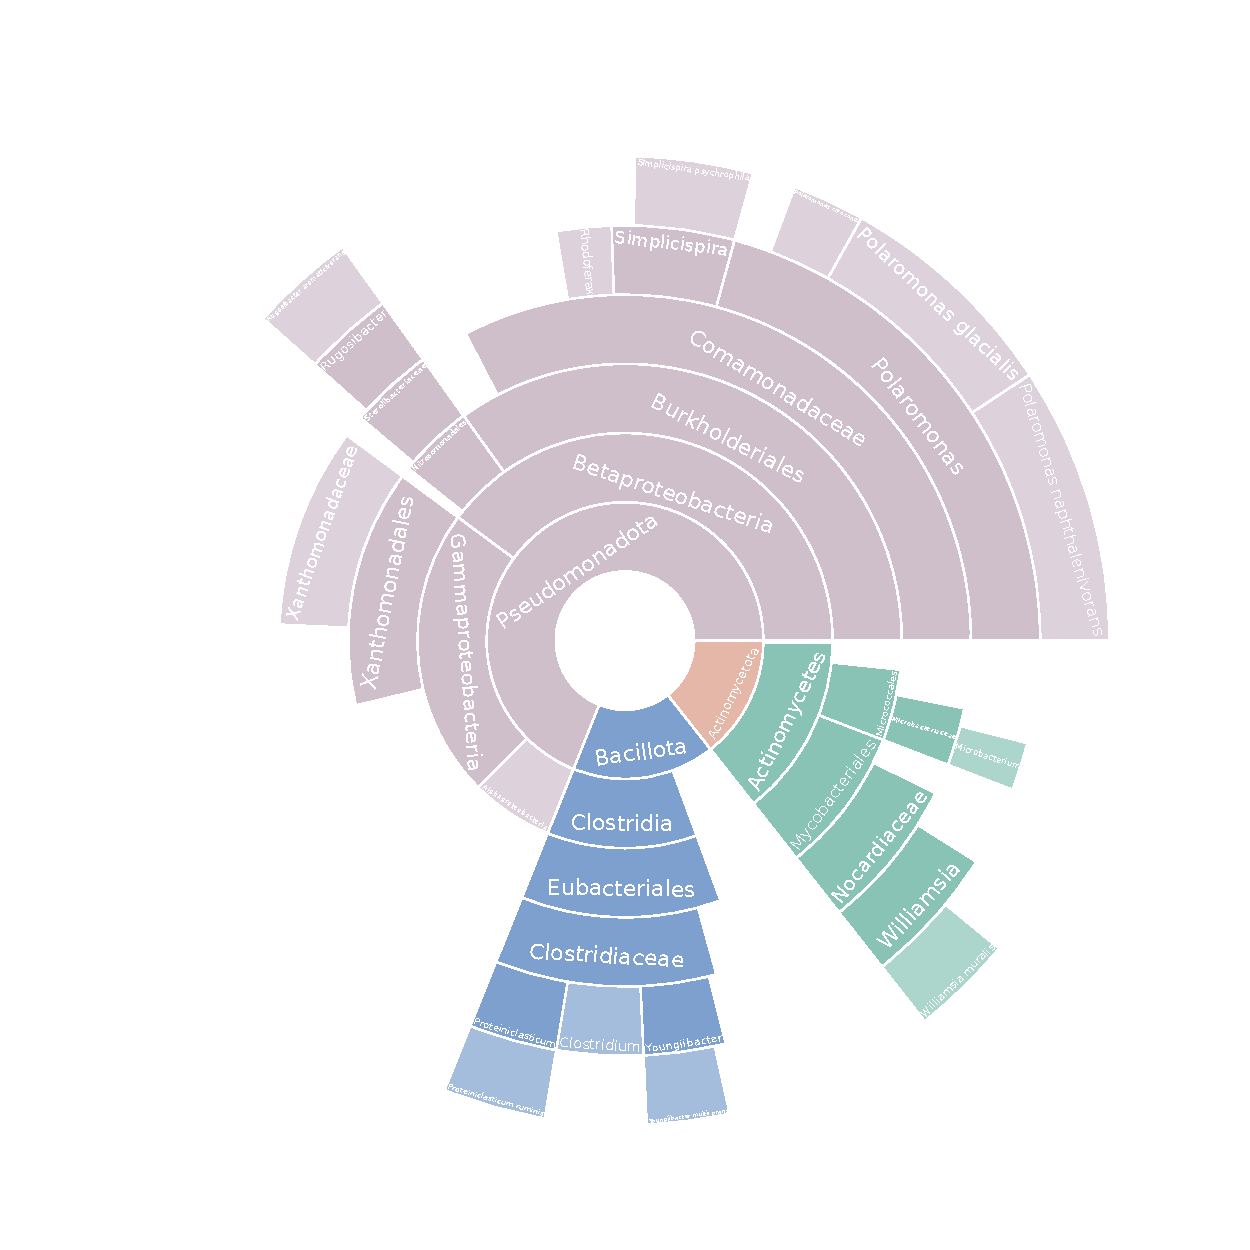
\includegraphics[width=0.9\linewidth]{images/pipeline/core_Impactadas.pdf}
    \caption{Gráfico jerárquico generado para el grupo de muestras categorizadas como No impactadas}
    \label{fig:pipeline-core}
\end{figure}

\subsubsection{Indices de diversidad}
Este módulo solo se ejecutara si el parámetro \textit{diversity.run} es ``ON'' en el archivo de configuración. 
Para poder ejecutarlo se requiere que el usuario haya ingreado grupos asociados a las muestras en el archivo de metadata.

El cálculo de los índices de diversidad se realizará utilizando el paquete \textit{vegan} de R.
La entrada de este módulo es el archivo resumen de blastn obtenido en el módulo anterior (\textit{merge\_blast\_out}) que contiene en las columnas las muestras y en las filas las especies, y  en la intersección la cantiadad de lecturas asociadas.
Además del archivo resumen de blast, este módulo requiere los grupos asociados a las muestras en formato diccionario (proveniente del archivo de configuración).

Mediante la función \textit{diversity} se calculan los índices de Simpson y Shannon, y mediante la función \textit{estimateR} se calcula el índice de Chao1.
El output de este módulo es una carpeta llamada \textit{diversity} que contiene un archivo csv con los valores de los índices de diversidad calculados para cada muestra y grupo ingresado (\textit{diversity\_index.csv}). 
Mediante ggplot se representa la información de los índices de diversidad en un gráfico de cajas y bigotes (\textit{boxplot.pdf}).

\subsubsection{Predicción funcional}
Este módulo solo se ejecutara si el parámetro \textit{functional\_prediction.run} es ``ON'' en el archivo de configuración. 
Para poder ejecutar la diferenciación entre grupos se requiere que el usuario haya ingreado esta información en el archivo de metadata.

La predicción funcinoal se realizará mediante la herramienta PICRUSt2. 
Para disminuir los tiempos de ejecucción, se realizará la predicción por muestra y luego mediante un script en python se unirán los resultados en un solo archivo.
Para la búsqueda de vías metabólicas que presenten diferencias significativas entre grupos se utilizará la herramienta Lefse (\hl{valor de normalización}).

El output de este módulo es una carpeta llamada \textit{functional\_prediction} que contiene los siguientes directorios:
\begin{itemize}
    \item \textit{picrust2\_out}: Directorio con los resultados de la predicción funcional por muestra. Contiene los siguientes directorios:
    \begin{itemize}
        \item \textit{EC\_metagenome\_out}: Directorio con los resultados de la predicción de las enzimas EC.
        \item \textit{KO\_metagenome\_out}: Directorio con los resultados de la predicción de los genes KO.
        \item \textit{Pathways\_out}: Directorio con los resultados de la predicción de las vías metabólicas.
    \end{itemize}
    \item \textit{KO.csv}: Archivo resumen con los resultados de la predicción de los genes KO para todas las muestras.
    \item \textit{EC.csv}: Archivo resumen con los resultados de la predicción de las enzimas EC para todas las muestras.
    \item \textit{Pathways.csv}: Archivo resumen con los resultados de la predicción de las vías metabólicas para todas las muestras.
    \item Gráfico de barras con vías metabólicas que presentan diferencias significativas entre grupos
    \end{itemize}
\subsubsection{Ejecución del flujo de trabajo}

\subsubsection{Escritura en la base de datos}
archivo que hace params

% \begin{figure}[H]
%     \centering
%     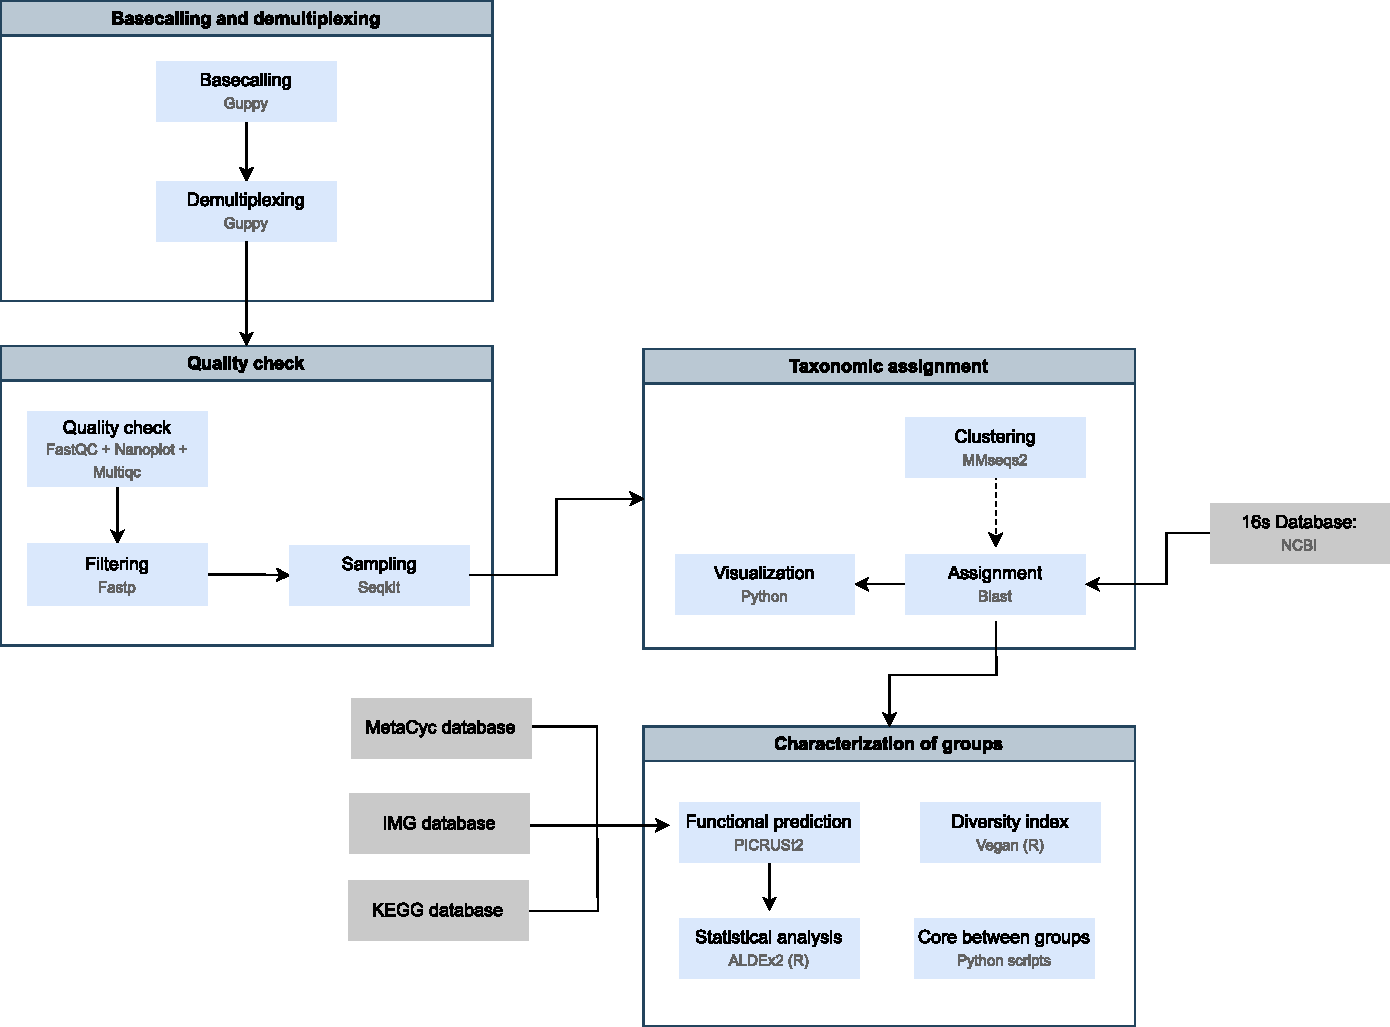
\includegraphics[width=1\linewidth]{images/pipeline.pdf}
%     \caption{Bioinformatics pipeline}
%     \label{fig:pipeline}
% \end{figure}


\hl{Desarrollo de contenedores o conda enviroments}
Para la reproducibilidad del flujo de trabajo se cuenta con dos \hl{executers}: Conda y \hl{Singularity}    .

\section{Base de datos}
\hl{añadir cardinalidad}
\begin{figure}[H]
    \centering
    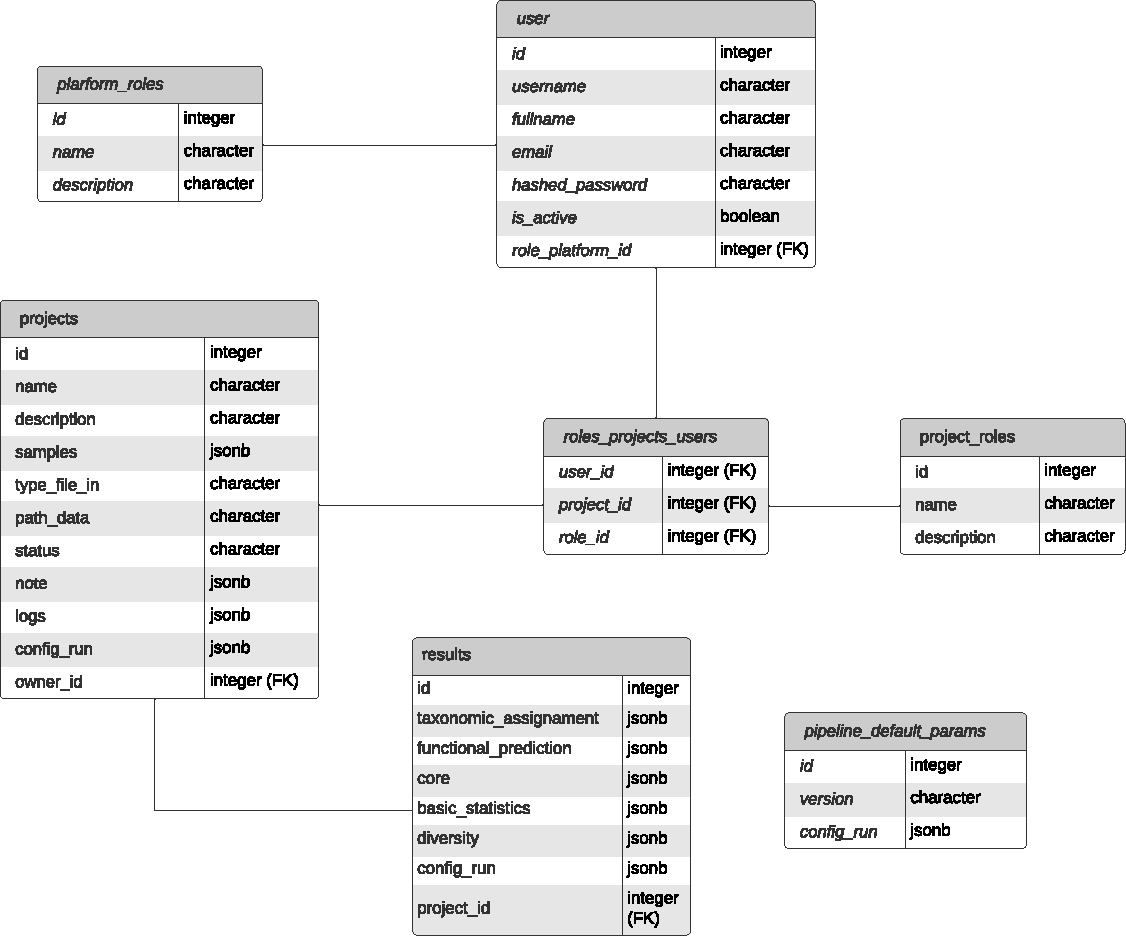
\includegraphics[width=1\linewidth]{images/nanotax-db.pdf}
    \caption{Base de datos}
    \label{fig:nanotax-db}
\end{figure}


% \subsection{Tabla de Usuarios}
% \begin{table}[H]
%     \begin{tabular}{|l|l|l|l|l|}
%         \hline
%         campo              & tipo de dato & descripción       & PK & FK \\ \hline
%         id                 & int          & ID                & Si & No \\ \hline
%         username           & str          & Nombre de usuario & No & No \\ \hline
%         fullname           & str          & Nombre completo   & No & No \\ \hline
%         email              & str          & Email             & No & No \\ \hline
%         hasshed\_password  & str          &                   & No & No \\ \hline
%         is\_active         & bool         &                   & No & No \\ \hline
%         role\_platform\_id & int          &                   & No & Si \\ \hline
%     \end{tabular}
%     \caption{Tabla Users}
%     \label{tab:db-users}
% \end{table}
% \subsection{Roles de la plataforma}
% \begin{table}[H]
%     \begin{tabular}{|l|l|l|l|l|}
%         \hline
%         campo       & tipo de dato & descripción                         & PK & FK \\ \hline
%         id          & int          & ID                                  & Si & No \\ \hline
%         name        & str          & Nombre del rol (admin / basic user) & No & No \\ \hline
%         description & str          & Descripción del rol                 & No & No \\ \hline
%     \end{tabular}
%     \caption{Tabla PlatformRole}
%     \label{tab:db-platformRole}
% \end{table}
% \subsection{Projectos}


% \begin{table}[H]
%     \begin{tabular}{|l|l|l|l|}
%         \hline
%         campo          & tipo de dato          & descripción                                                                                                                       & FK \\ \hline
%         id             & int (PK)              & ID                                                                                                                                & No \\ \hline
%         name           & str                   & Nombre del projecto                                                                                                               & No \\ \hline
%         description    & str                   & Descripción del proyecto                                                                                                          & No \\ \hline
%         samples        & JSON/dict{[}str,any\} & \begin{tabular}[c]{@{}l@{}}Metadata de las muestras. Puede contener como claves: \\ Barcode, Sample, Group, Subgroup\end{tabular} & No \\ \hline
%         colaboration   & str                   & ???                                                                                                                               & No \\ \hline
%         type\_file\_in & str                   & Tipo de archivo a procesar (POD5, FASTQ, CSV, FASTA)                                                                              & No \\ \hline
%         path\_data     & str                   & Ruta en el servidor donde se almacenaran los archivos de entrada                                                                  & No \\ \hline
%         status         & str                   & \begin{tabular}[c]{@{}l@{}}Estado del proyecto en ejecución \\ (upload\_data / running / failed / finish)\end{tabular}            & No \\ \hline
%         note           & JSON/dict{[}str,any\} & \begin{tabular}[c]{@{}l@{}}Información sobre el proyecto \\ (cantidad de muestras total, procesadas y descartadas)\end{tabular}   & No \\ \hline
%         logs           & JSON/dict{[}str,any\} & Logs                                                                                                                              & No \\ \hline
%         owner\_id      & int                   & Id del usuario que sube el proyecto                                                                                               & Si \\ \hline
%     \end{tabular}
%     \caption{Tabla de Proyectos}
%     \label{tab:db-projects}
% \end{table}

% \subsection{Roles del Proyecto}
% \begin{table}[H]
%     \begin{tabular}{|l|l|l|l|}
%         \hline
%         campo       & tipo de dato & descripción                               & FK \\ \hline
%         id          & int (PK)     & ID                                        & No \\ \hline
%         name        & str          & Nombre del rol (leer, escribir, eliminar) & No \\ \hline
%         description & str          & Descripción del rol                       & No \\ \hline
%     \end{tabular}
%     \caption{Tabla de Roles de Proyectos}
%     \label{tab:db-role_projects}
% \end{table}
% \subsection{Roles Projectos y Usuarios}
% \begin{table}[H]
%     \begin{tabular}{|l|l|l|l|}
%     \hline
%     campo       & tipo de dato & descripción                                       & FK \\ \hline
%     user\_id    & int (PK)     & ID del usuario                                    & Si \\ \hline
%     project\_id & int (PK)     & ID del proyecto                                   & Si \\ \hline
%     role\_id    & int (PK)     & Rol del usuario dentro del proyecto en especifico & Si \\ \hline
%     \end{tabular}
%     \caption{Tabla de Roles Proyectos y Usuarios}
%     \label{tab:db-role_projects_users}
%     \end{table}

% \subsection{Resultados}
% \begin{table}[H]
%     \small
%     \begin{tabular}{|l|l|l|l|}
%     \hline
%     campo                  & tipo de dato           & descripción                                                                                                                                              & FK \\ \hline
%     id                     & int                    & ID                                                                                                                                                       & No \\ \hline
%     taxonomic\_assignament & JSON/dict{[}str,any{]} & \begin{tabular}[c]{@{}l@{}}Assignación taxonomica por muestra y por nivel taxonómico\\ (especie, genero, familia, orden, clase y filo)\end{tabular}      & No \\ \hline
%     functional\_prediction & JSON/dict{[}str,any{]} & \begin{tabular}[c]{@{}l@{}}Resultados de la predicción funcional por muestra y \\ por categoría funcional (EC, Pathways, KO)\end{tabular}                & No \\ \hline
%     core                   & JSON/dict{[}str,any{]} & Cantidad de lecturas/porcentaje compartido entre los grupos                                                                                              & No \\ \hline
%     basic\_statistics      & JSON/dict{[}str,any{]} & \begin{tabular}[c]{@{}l@{}}Estadísticas básicas de las muestras\\ (Total de lecturas procesadas y sin procesar,\\ calidad y largo promedio)\end{tabular} & No \\ \hline
%     diversity              & JSON/dict{[}str,any{]} & \begin{tabular}[c]{@{}l@{}}Calculo de los indices de diversidad\\ (Shannon, Simpson, Chao2)\end{tabular}                                                 & No \\ \hline
%     config\_run            & JSON/dict{[}str,any{]} & Parámetros personalizados por el usuario                                                                                                                 & No \\ \hline
%     project\_id            & int                    & ID del proyecto                                                                                                                                          & Si \\ \hline
%     \end{tabular}
%     \caption{Tabla de Resultados}
%     \label{tab:db-results}
%     \end{table}

\newpage
\section{Aplicación Web}
Se desarrollo una aplicación web mediante Vue3 y FastAPI que permite al usuario subir sus archivos de secuenciación y metadata. 
Con esto el usuario puede abstraerse de tener conocimiento en línea de comando o ejecución de heramientas bioinformaticas y/o flujos de trabajo, 
ya que mediante la interfaz web el usuario solo debe seleccionar los análisis que desea realizar.
La información ingresada por el usuario es guardada en la base de datos y mediante un script se generan los parámetros necesarios para la ejecución del flujo de trabajo.
Una vez el pipeline termina de ejecutarse se escriben los resultados en la base de datos. 
La plataforma lee esta información directa de la base de datos y despliega los resultados en forma de tablas y gráficos en la sección de análisis.

\hl{script que genera los parametros de ejecución del flujo de trabajo} 

A continuación se detalla cada una de las vistas de la aplicación web y su funcionalidad.
% \subsection{Middleware}
% \subsection{Security}

\subsection{Login}
Al ingresar en la página de Login, el usuario deberá ingresar su nombre de usuario y contraseña.
En caso de que los datos sean correctos será redireccionado a la página de proyectos (Ver sección \ref{projects}).
En caso de que los datos sean incorrectos se mostrará un mensaje de error \textit{“Usuario o contraseña incorrectos”} y deberá ingresar sus credenciales nuevamente.


\begin{figure}[ht]
    \centering
    \begin{subfigure}[b]{0.45\textwidth}
        \centering
        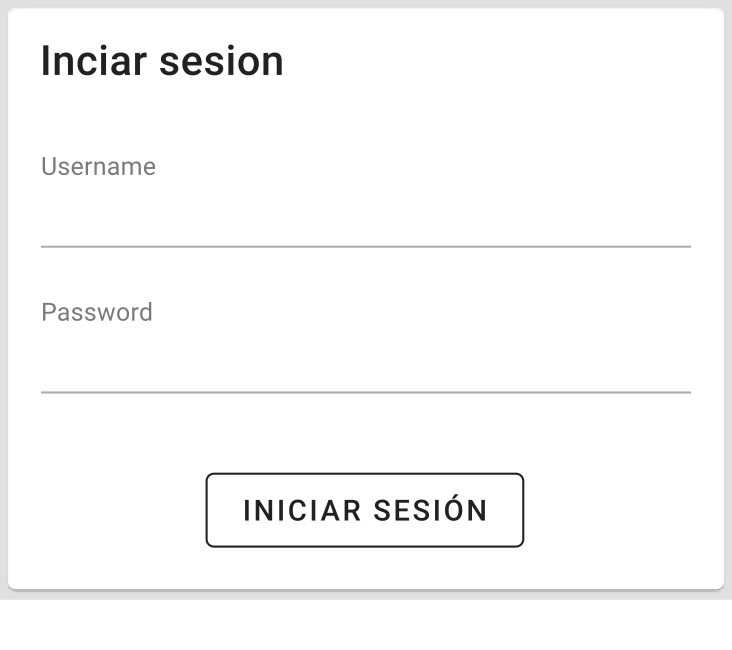
\includegraphics[width=\textwidth]{images/app/login.png}
        \caption{Vista de inicio de sesión por defecto \newline}
        \label{fig:app-login_default}
    \end{subfigure}
    \hfill
    \begin{subfigure}[b]{0.45\textwidth}
        \centering
        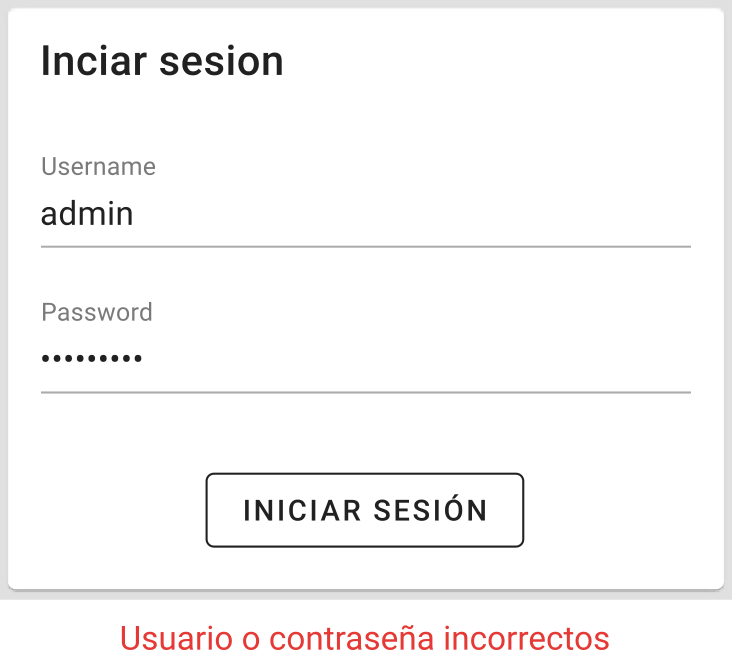
\includegraphics[width=\textwidth]{images/app/login-error.png}
        \caption{Vista de inicio de sesión con mensaje de error al ingresar credenciales inválidas}
        \label{fig:app-login_error}
    \end{subfigure}
    \caption{Vista de Inicio de sesión}
    \label{fig:app-login}
\end{figure}

\hl{Registrarse - vista}
\subsection{Navbar?}

\subsection{Cambio de contraseña}
Una vez que el usuario validó sus credenciales va a poder acceder a la vista de cambio de contraseña a través de la barra de navegación (Figura~\ref{fig:app-change-psw_default}).



Para realizar el cambio de contraseña, deberá ingresar su contraseña actual y su nueva contraseña dos veces.
En caso de que la contraseña sea cambiada con éxito se mostrará el mensaje \textit{“Contraseña cambiada con exito“} (Figura~\ref{fig:app-change-psw-success}).


\begin{figure}[H]
    \centering
    \begin{subfigure}[b]{0.45\textwidth}
        \centering
        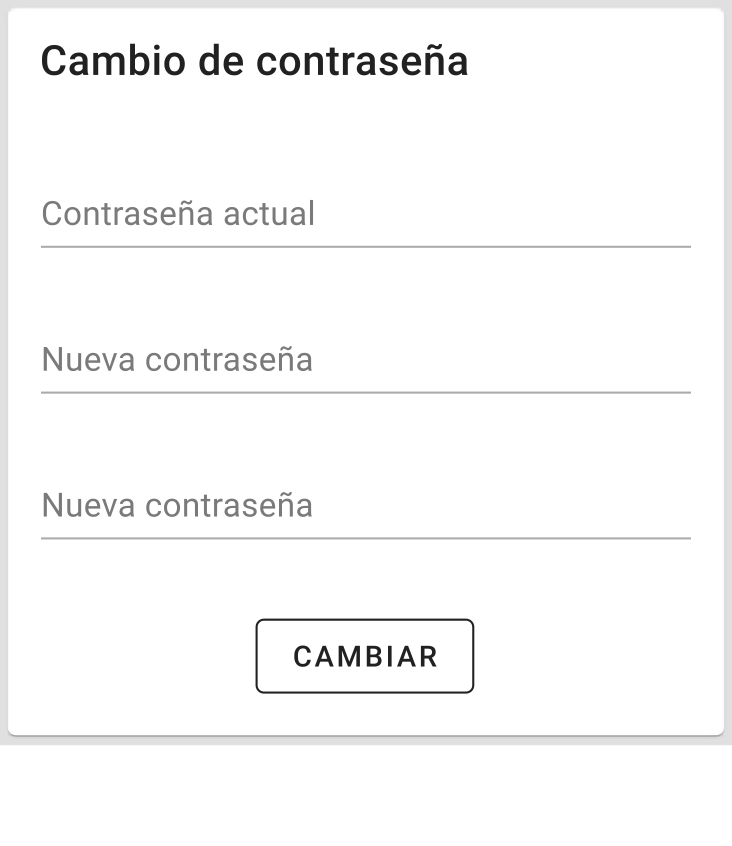
\includegraphics[width=\textwidth]{images/app/change-psw-def.png}
        \caption{Vista de cambio de contraseña por defecto \newline}
        \label{fig:app-change-psw_default}
    \end{subfigure}
    \hfill
    \begin{subfigure}[b]{0.45\textwidth}
        \centering
        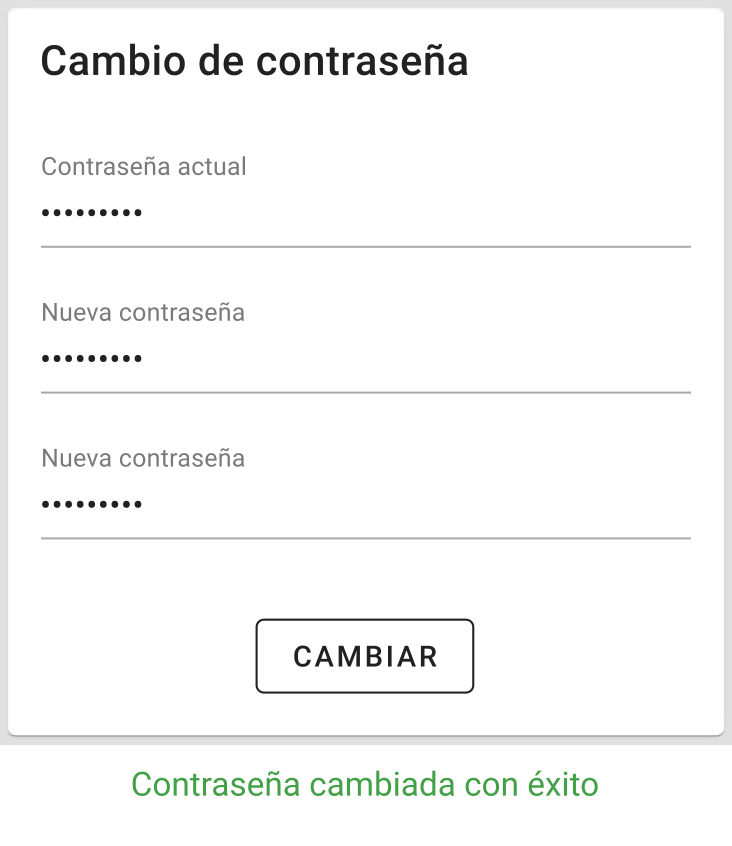
\includegraphics[width=\textwidth]{images/app/change-psw-sucess.png}
        \caption{Vista de cambio de contraseña realizado con exito}
        \label{fig:app-change-psw-success}
    \end{subfigure}
    % \caption{Vista de Cambio de contraseña (I)}
    \label{fig:app-change-psw-1}
\end{figure}
En caso de que la contraseña actual sea incorrecta se mostrará el mensaje de error  \textit{“Contraseña incorrecta”} (Figura~\ref{fig:app-change-psw_error-1}).
En caso de que las contraseñas nuevas no coincidan se mostrará el mensaje de error \textit{“Las contraseñas no coinciden”} (Figura~\ref{fig:app-change-psw_error-2})
\begin{figure}[H]
    \centering
    \begin{subfigure}[b]{0.45\textwidth}
        \centering
        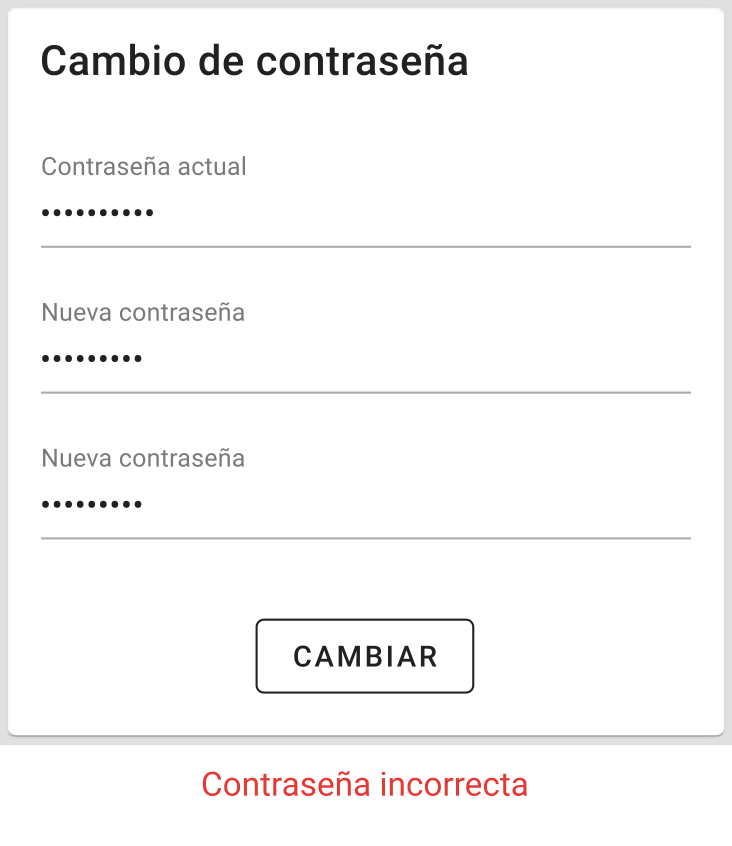
\includegraphics[width=\textwidth]{images/app/change-psw-error1.png}
        \caption{Vista de cambio de contraseña al ingresar contraseña incorrecta}
        \label{fig:app-change-psw_error-1}
    \end{subfigure}
    \hfill
    \begin{subfigure}[b]{0.45\textwidth}
        \centering
        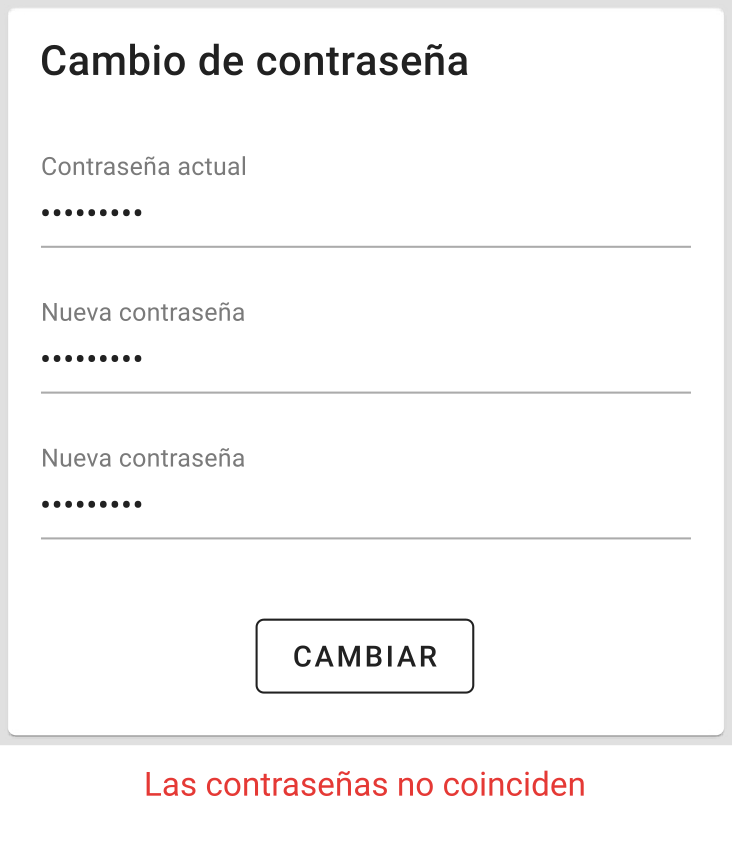
\includegraphics[width=\textwidth]{images/app/change-psw-error2.png}
        \caption{Vista de cambio de contraseña al ingresar contraseñas que no coinciden}
        \label{fig:app-change-psw_error-2}
    \end{subfigure}
    % \caption{Vista de Cambio de contraseña (II)}
    \label{fig:app-change-psw-2}
\end{figure}

En el caso de que la nueva contraseña no cumpla los críterios de seguridad (longitud mínima de 8 caracteres y al menos un número) se mostrará el mensaje de error  \textit{“La contraseña debe tener al menos 8 caracteres / La contraseña debe tener al menos un número”} (Figura~\ref{fig:app-change-psw_error-1}).
\begin{figure}[H]
    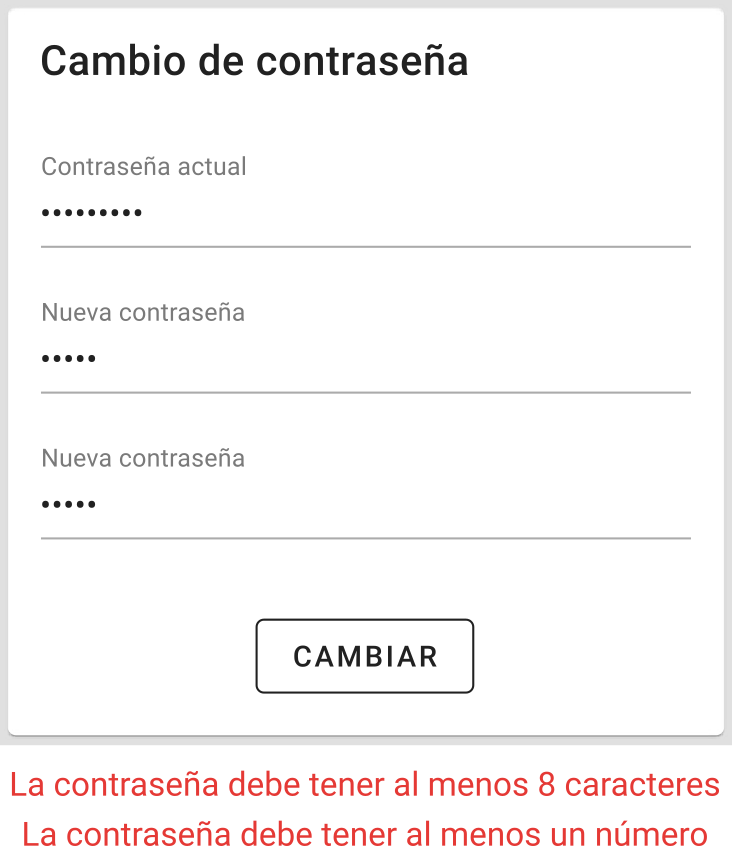
\includegraphics[width=0.45\linewidth]{images/app/change-psw-error3.png}
    \captionsetup{justification=raggedright, width=0.45\linewidth, singlelinecheck=off}

    % \captionsetup{width=0.45\linewidth}
    \caption{Vista de cambio de contraseña al ingresar una nueva contraseña que no cumple con los críterios de seguridad}
    \label{fig:app-change-psw_error-3}
\end{figure}

% \begin{figure}[H]
%     \centering
%     \begin{subfigure}[b]{0.4\textwidth}
%         \centering
%         \includegraphics[width=\textwidth]{images/app/chage-psw-def.png}
%         \caption{a}
%         \label{fig:subfig1}
%     \end{subfigure}
%     \hfill
%     \begin{subfigure}[b]{0.4\textwidth}
%         \centering
%         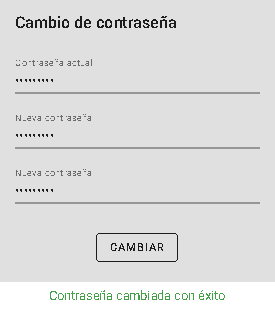
\includegraphics[width=\textwidth]{images/app/chage-psw-sucess.png}
%         \caption{b}
%         \label{fig:subfig2}
%     \end{subfigure}

%     \vskip\baselineskip

%     \begin{subfigure}[b]{0.4\textwidth}
%         \centering
%         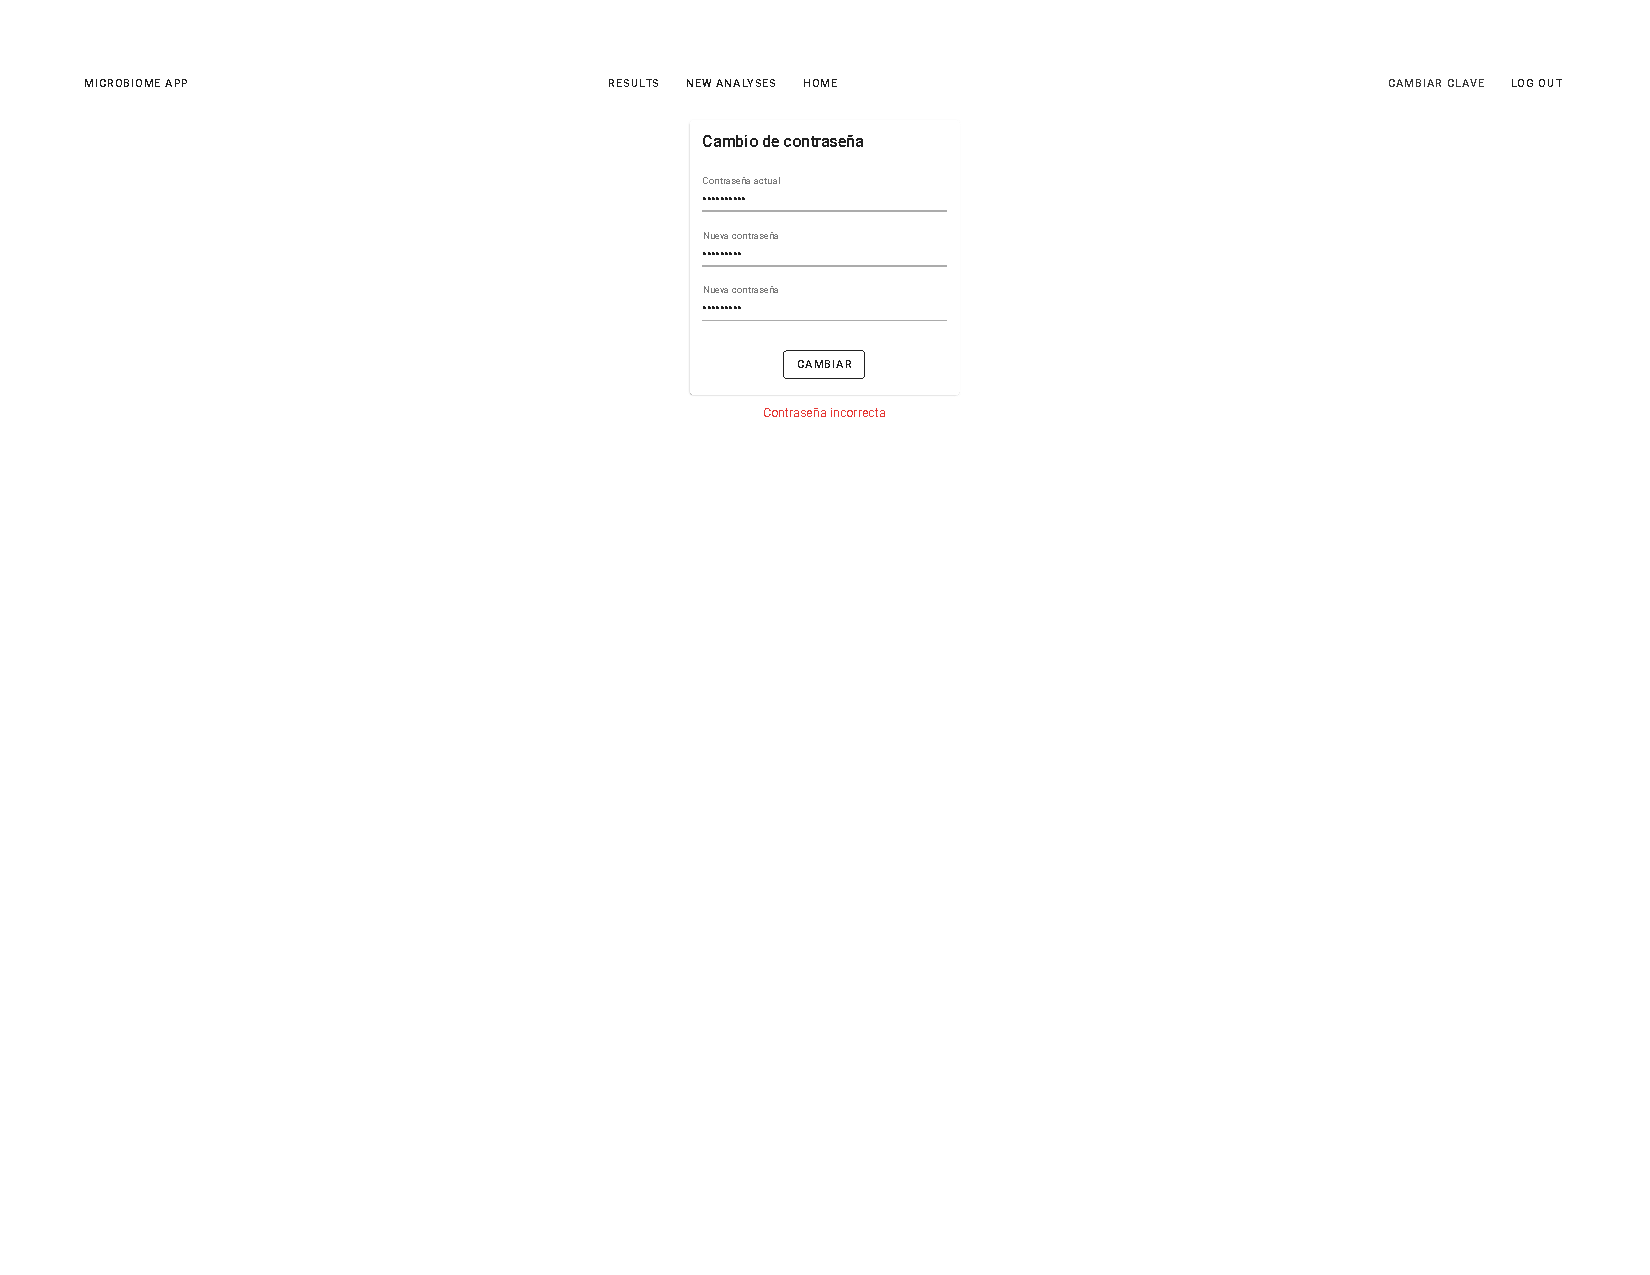
\includegraphics[width=\textwidth]{images/app/chage-psw-error1.png}
%         \caption{c}
%         \label{fig:subfig3}
%     \end{subfigure}
%     \hfill
%     \begin{subfigure}[b]{0.4\textwidth}
%         \centering
%         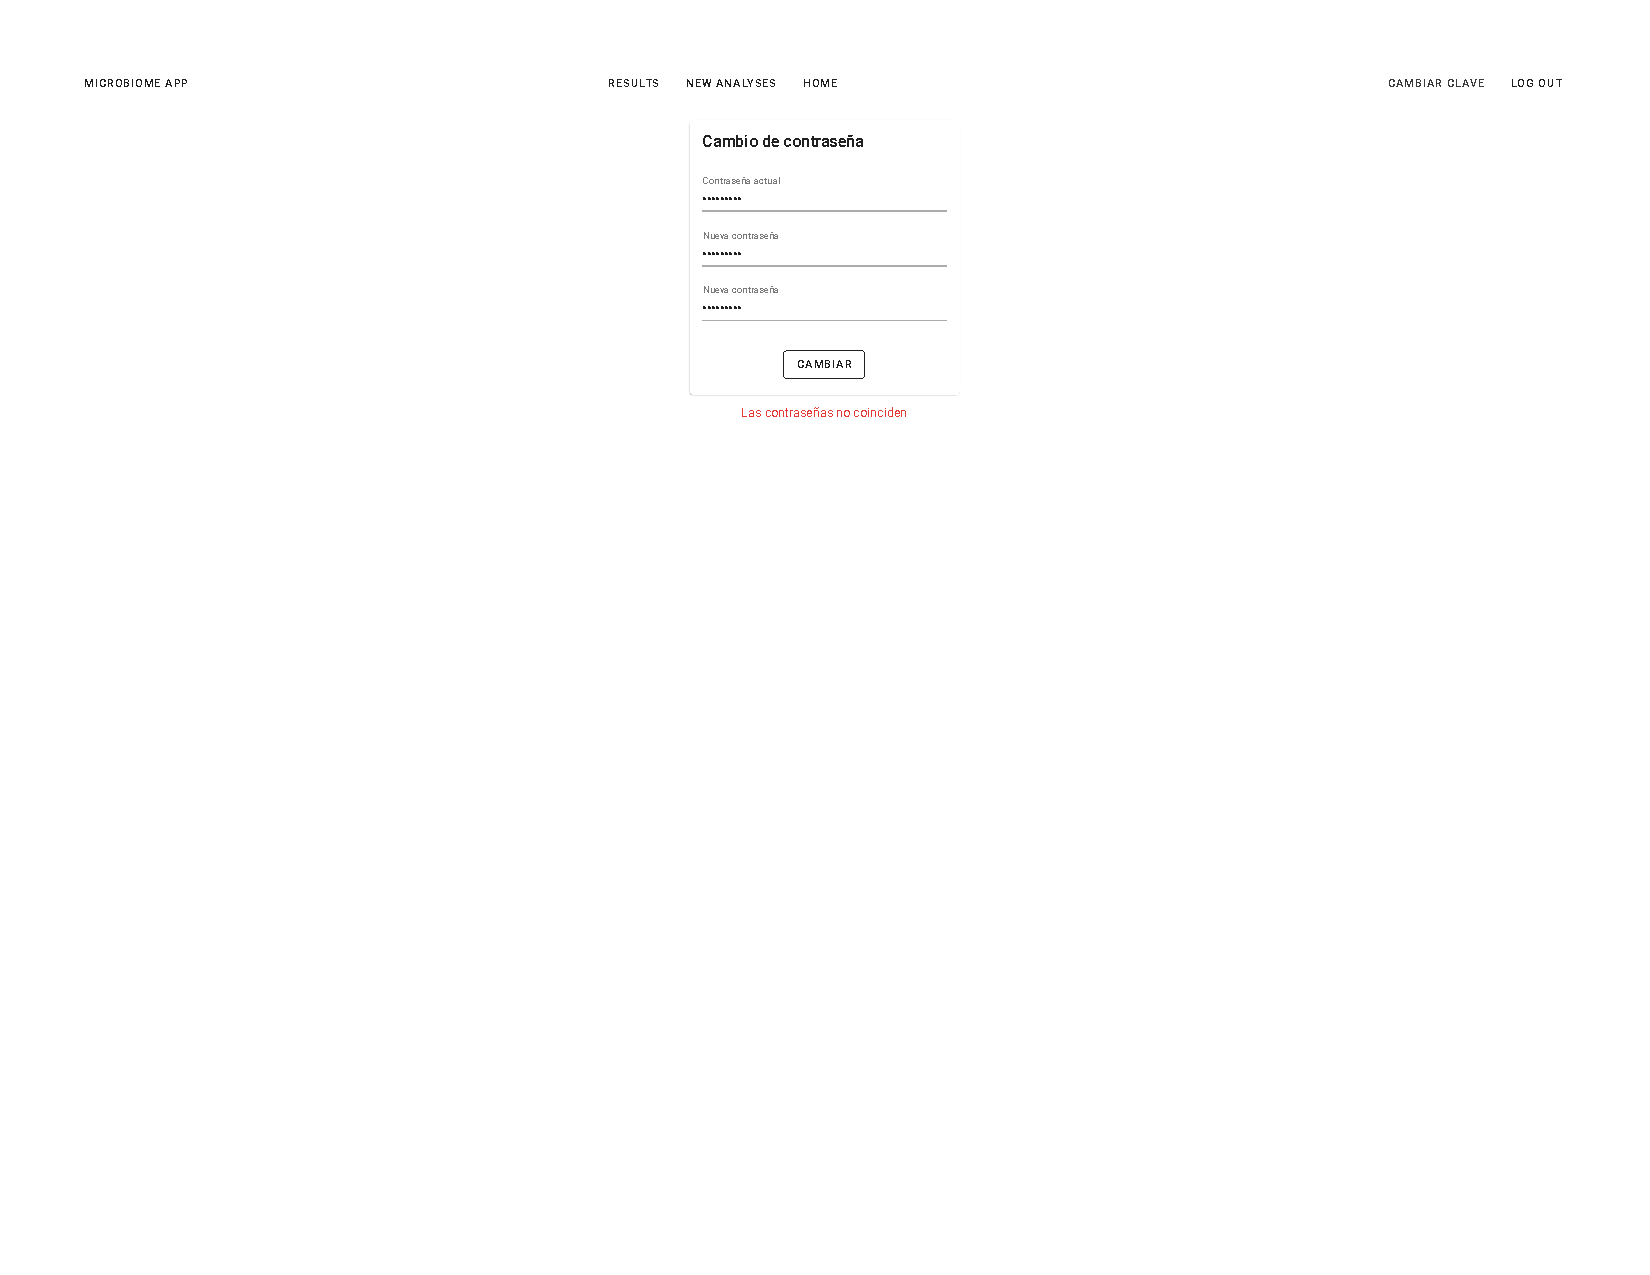
\includegraphics[width=\textwidth]{images/app/chage-psw-error2.png}
%         \caption{d}
%         \label{fig:subfig4}
%     \end{subfigure}

%     \vskip\baselineskip

%     \begin{subfigure}[b]{0.4\textwidth}
%         \centering
%         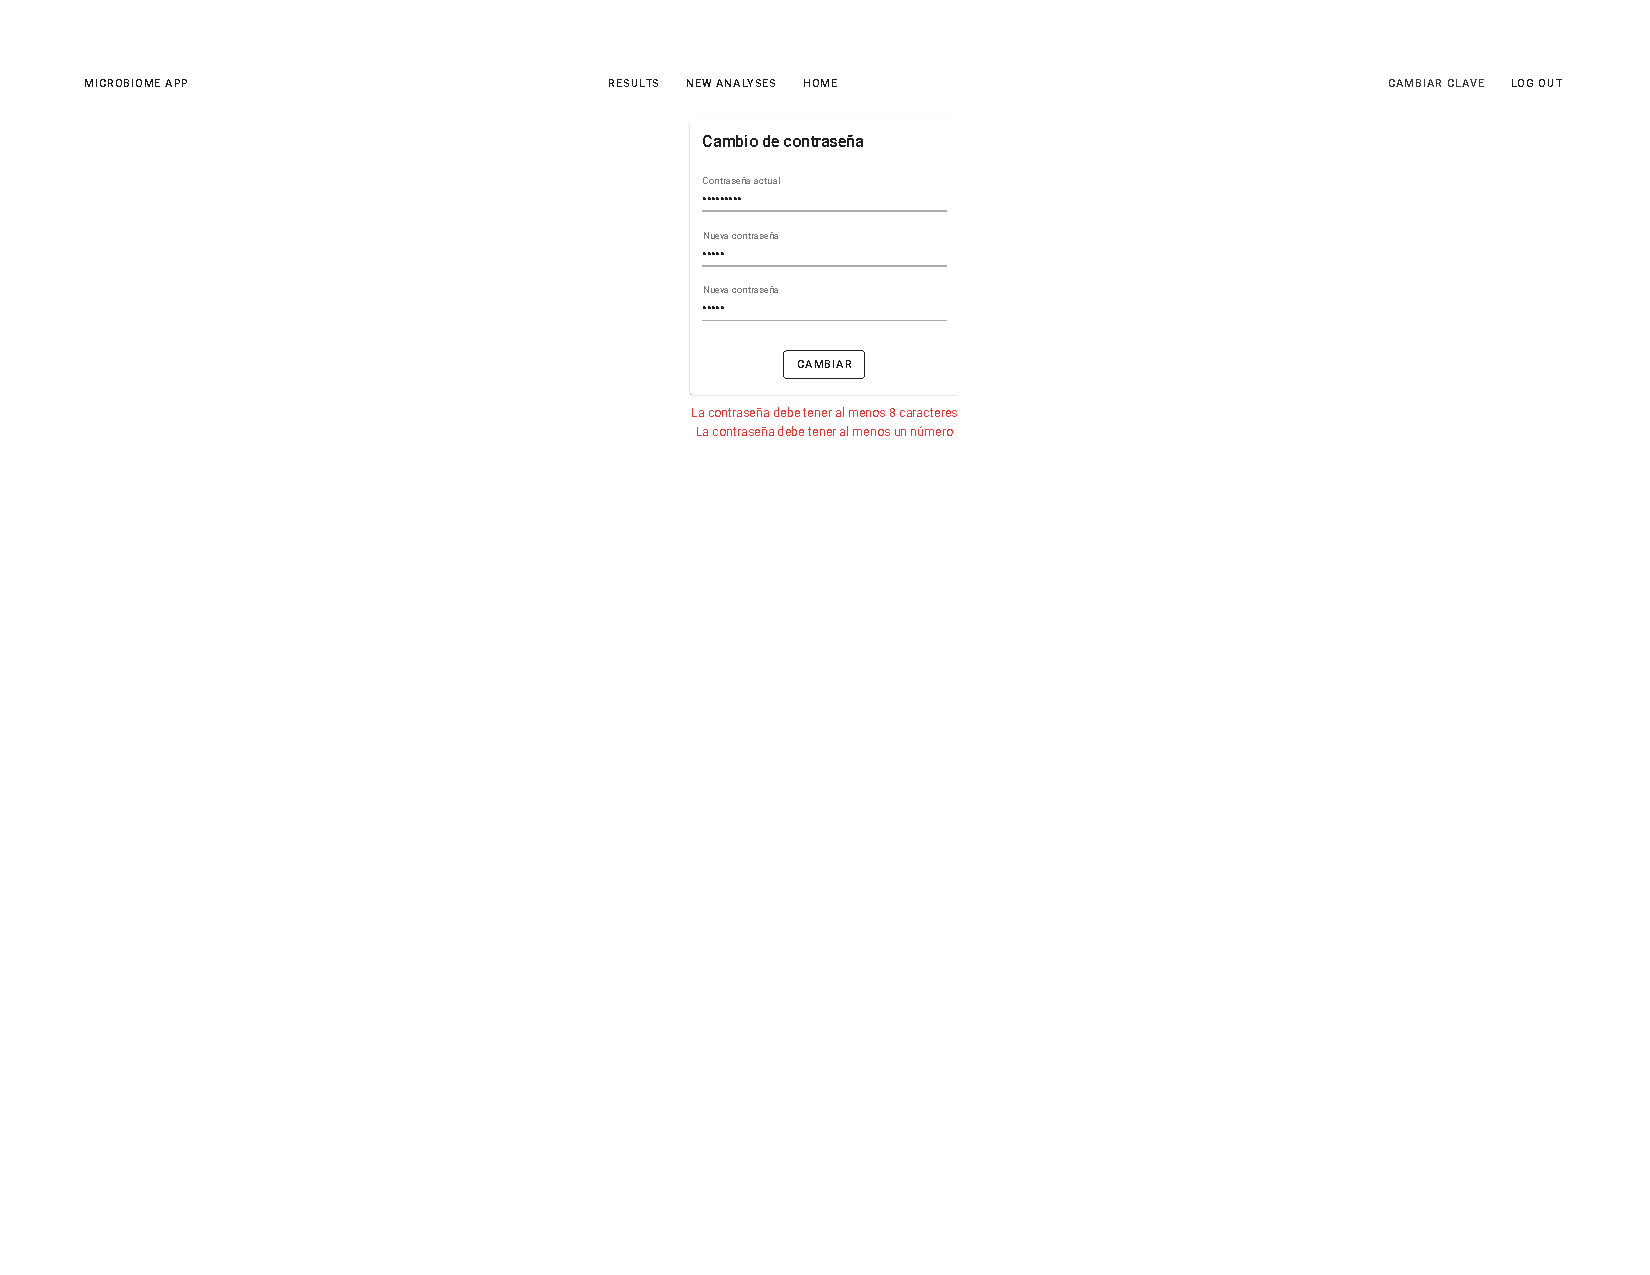
\includegraphics[width=\textwidth]{images/app/chage-psw-error3.png}
%         \caption{e}
%         \label{fig:subfig5}
%     \end{subfigure}
    
%     \caption{Título de la figura principal}
%     \label{fig:main}
% \end{figure}


\subsection{Nuevo análisis}
En esta sección el usuario deberá ingresar la información del proyecto, datos de secuenciación, y metadata para poder realizar los análisis. 
El usuario deberá rellenar la información básica del proyecto como, nombre, descripción, tipo de archivos y mediante un archivo en formato (XLXS) deberá ingresar la información de las muestras. %, como nombre de archivo, nombre de la muestra, barcode (opcional) y grupo (opcional).
Los datos de secuenciación se debe subir a algún directorio del drive del usuario y se debe dar acceso a la cuenta \textit{nanotax.catg@gmail.com}.
La figura~\ref{fig:app-new-analysis-def} presenta la vista inicial de la sección de Nuevo análisis.

\begin{figure}[H]
    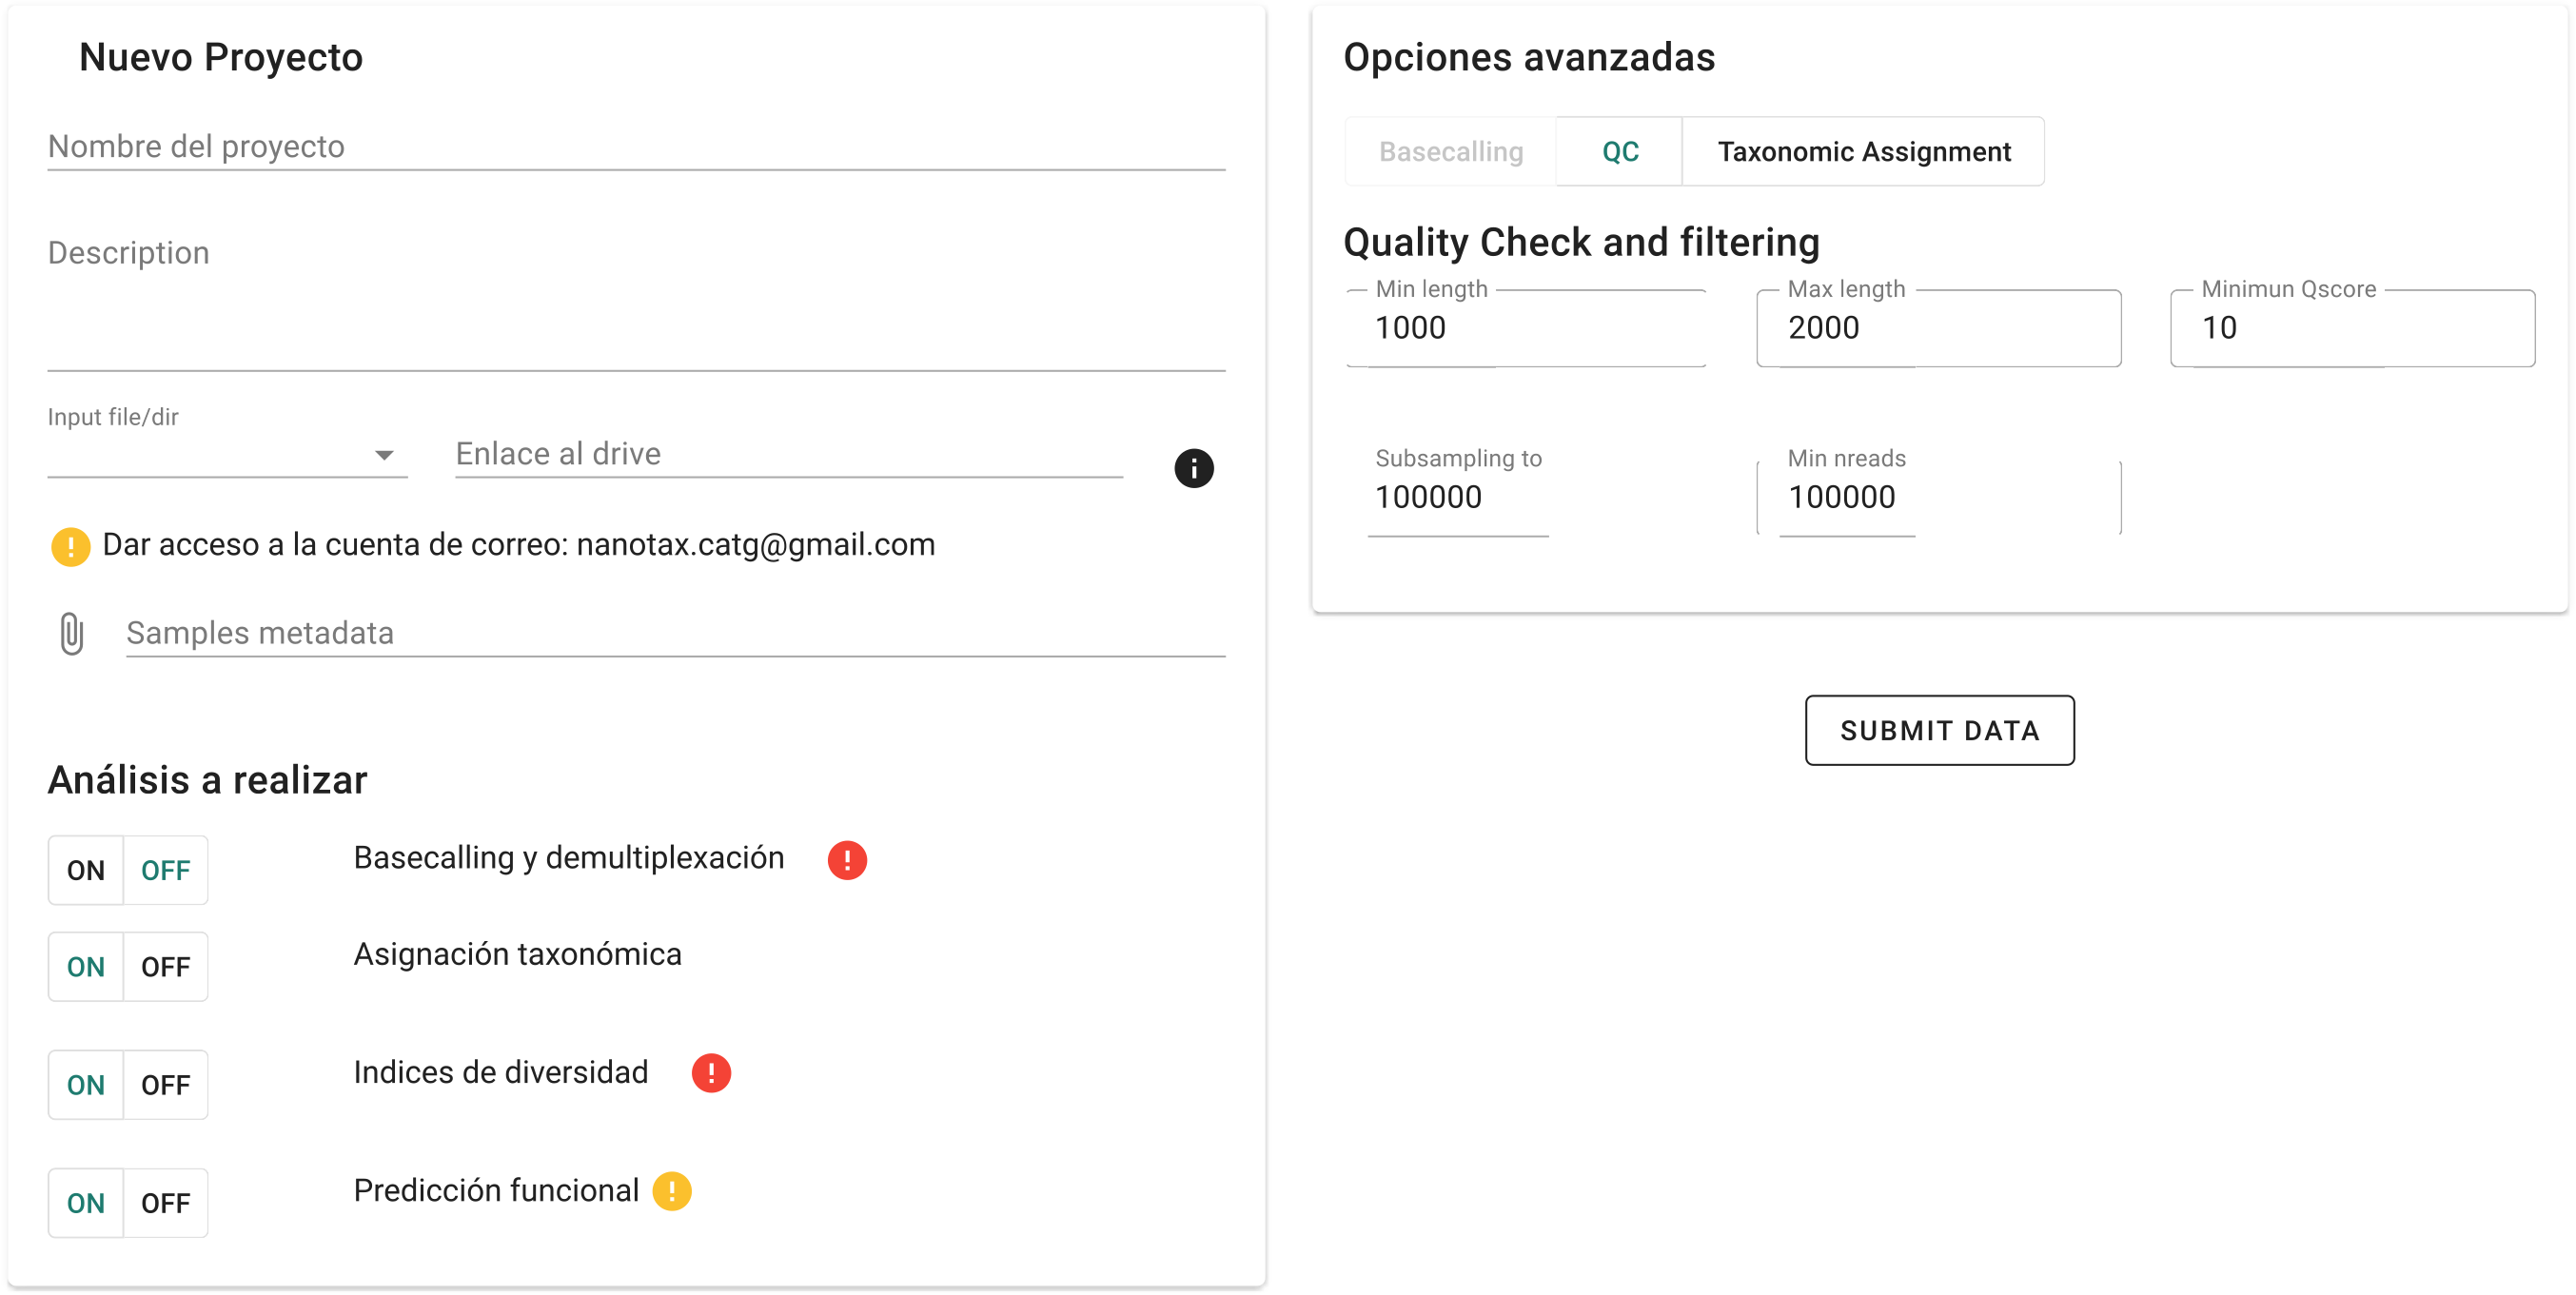
\includegraphics[width=1\linewidth]{images/app/newAnalysis/new-analysis-def.png}
    % \captionsetup{justification=raggedright, width=0.45\linewidth, singlelinecheck=off}

    % \captionsetup{width=0.45\linewidth}
    \caption{Vista por defecto de Nuevo análisis}
    \label{fig:app-new-analysis-def}
\end{figure}


A continuación se describen los datos que el usuario debe rellenar:

\begin{itemize}
    \item Nombre: Nombre del proyecto a utilizar en la plataforma (sección de visualización de proyectos y resultados).
    \item Descripción (opcional): Descripción del proyecto, campo opcional.
    \item Tipo de archivo a subir (POD5, FASTQ): Archivos de secuenciación que se procesarán:
    \begin{itemize}
        \item POD5: En caso de querer comenzar desde el proceso de basecalling y demultiplexación de las muestras.
        \item FASTQ: En caso de querer saltarse el paso de basecalling y demultiplexación e iniciar directamente con el control de calidad y asignación taxonómica.
    \end{itemize}
    \item Archivo de metadata en formato XLXS con las siguientes columnas para cada muestra:
    \begin{itemize}
        \item file: nombre del archivo subido al drive (obligatorio)
        \item sample: identificador de la muestra (obligatorio)
        \item barcode (opcional): barcode que identifica la muestra (en caso de querer realizar basecalling y demultiplexación)
        \item group (opcional): groupo al que pertenece cada muestra (en caso de querer hacer diferenciación entre grupos)
        \item \hl{subgroup: subgrupo al que pertenece cada muestra (en caso de querer hacer diferenciación entre subgrupos)}
    \end{itemize}
    \item Análisis a realizar:
    \begin{itemize}
        \item Basecalling y demultiplexacion
        \item Asignación taxonomica
        \item Indices de diversidad
        \item Predicción funcional
    \end{itemize}
\end{itemize}


En el lado derecho de la vista se puede visualizar una sección de opciones avanzadas, donde el usuario puede modificar los parámetros por defecto en caso de que quiera modificar el comportamiento del pipeline (gigura~\ref{fig:app-new-analysis-def}). Esta información es seleccionados desde la base de datos la cual almacena los parámetros por defecto del flujo de trabajo.

\hl{Cabe destacar que en caso de que el directorio del drive no contenga la información necesaria, el proyecto se subirá correctamente y luego pasara a un estado de datos inválidos }
Los filtros y control de calidad se realizan siempre por lo que no aparecerá la opción en la lista de análisis.
Por defecto basecalling y demuliplexación se encuentra deshabilitado, en caso de que el usuario desee realizar este análisis deberá seleccionarlo, y al hacerlo se desbloqueará la sección de configuración de este análisis (Figura~\ref{fig:app-new-analysis-basecallingON}).



\begin{figure}[H]
    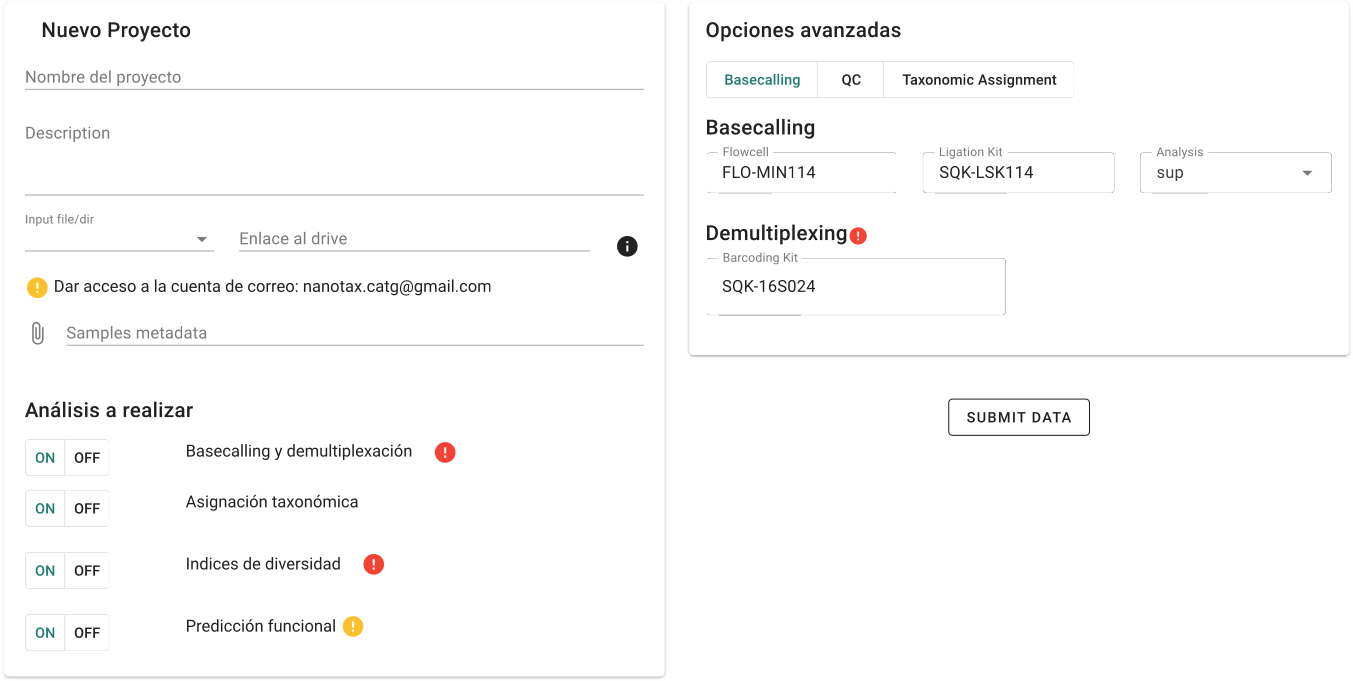
\includegraphics[width=1\linewidth]{images/app/newAnalysis/new-analysis-basecallingON.png}
    % \captionsetup{justification=raggedright, width=0.45\linewidth, singlelinecheck=off}

    % \captionsetup{width=0.45\linewidth}
    \caption{Vista de Nuevo análisis habilitando la opción de basecalling y demultiplexación}
    \label{fig:app-new-analysis-basecallingON}
\end{figure}
% La plataforma se encarga de verificar si el archivo de metadata cuenta con la información necesaria para realizar cada analisis. En caso de que el archivo de metadata no cuente con la información necesaria y el usuario desee realizar uno de esos analisis, se desplegara un mensaje de error al lado del análisis indicando que información se debe añadir en el archivo de metadata. Los parámetros que se pueden modificar son los siguientes:
% \begin{itemize}
%     \item Basecalling y demultiplexacion: Flowcell, kit de ligación y kit de barcoding utilizados durante la secuenciación. Modelo a utilizar para realizar el basecalling
%     \item QC: Longitud mínima y máxima en pares de bases de las lecturas, calidad mínima de las lecturas y cantidad de lecturas a utilizar para los análisis posteriores(subsampleo).
%     \item Predicción funcional: \hl{completar}
% \end{itemize}

% En la parte derecha del componente el usuario puede visualizar los parámetros por defecto y modificarlos en caso de que lo desee. 


Una vez que el usuario presione al botón \textit{Subir proyecto}, la plataforma realiza un proceso de validación para verificar que toda la información subida por el usuario sea correcta. En caso de no serla, la plataforma no permitirá subir el proyecto y podrá presentar alguno de los siguientes mensajes de error:
\begin{itemize}
    \item En caso de no completar el nombre del proyecto o el enlace al directorio del drive ambos campos pasarán a estar en color rojo (figura ~\ref{fig:app-new-analysis-type-file-error}).
    \item En caso de no seleccionar el tipo de archivo a subir, este campo pasará a estar en color rojo y se presentará el siguiente mensaje: \textit{Debe seleccionar el formato de los archivos de entrada} (figura ~\ref{fig:app-new-analysis-type-file-error}).
    \item En caso de seleccionar el formato de archivo \textit{POD5} y no haber seleccionado el proceso de basecalling y demultiplexación como inicio se presentará el mensaje: \textit{Al iniciar con basecalling debe subir los archivos POD5} (figura ~\ref{fig:app-new-analysis-type-file-error}).
    \item En caso de seleccionar el formato de archivo \textit{FASTQ} y haber seleccionado el proceso de basecalling y demultiplexación como inicio se presentará el mensaje: \textit{Al iniciar con QC o asignación taxonómica debe subir los archivos FASTQ} (figura ~\ref{fig:app-new-analysis-type-file-error}).
    \item En caso de que el archivo de metadata no cuente con todas las columnas necesarias se pueden presentar los siguientes mensajes de errores (figura ~\ref{fig:app-new-analysis-type-file-error}) \hl{no todos, solo lo que falte}:
    \begin{itemize}
        \item \textit{El archivo de metadata le falta la columna file}
        \item \textit{El archivo de metadata le falta la columna sample}
        \item \textit{El archivo de metadata le falta la columna barcode}: Solo en caso de seleccionar basecalling y demultiplexación como inicio del pipeline.
        \item \textit{El archivo de metadata le falta la columna group}: Solo en caso de querer realizar análisis por grupos (índices de diversidad).

    \end{itemize}
\end{itemize}


\begin{figure}[H]
    \centering
    \begin{subfigure}[b]{0.45\textwidth}
        \centering
        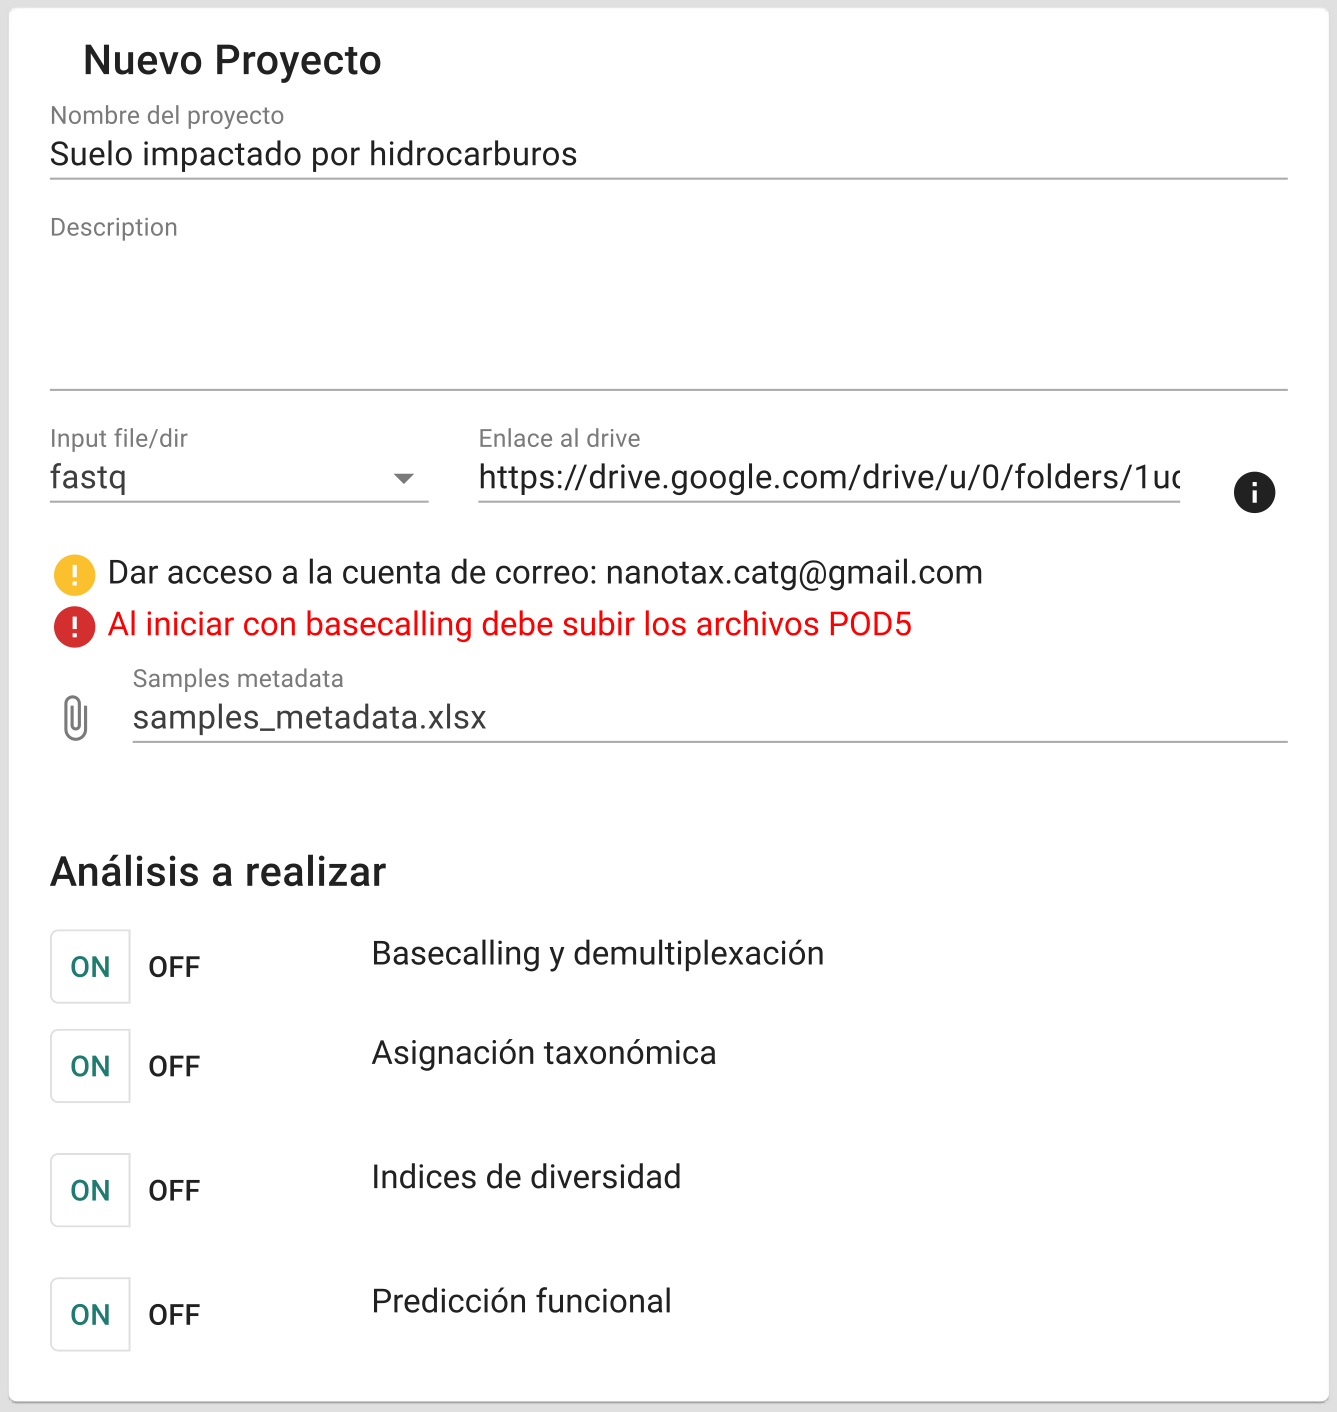
\includegraphics[width=\textwidth]{images/app/newAnalysis/pod5-error.png}
        \caption{Vista de nuevo análisis: Error al seleccionar el tipo del archivo}
        \label{fig:app-new-analysis-pod5-error}
    \end{subfigure}
    \hfill
    \begin{subfigure}[b]{0.45\textwidth}
        \centering
        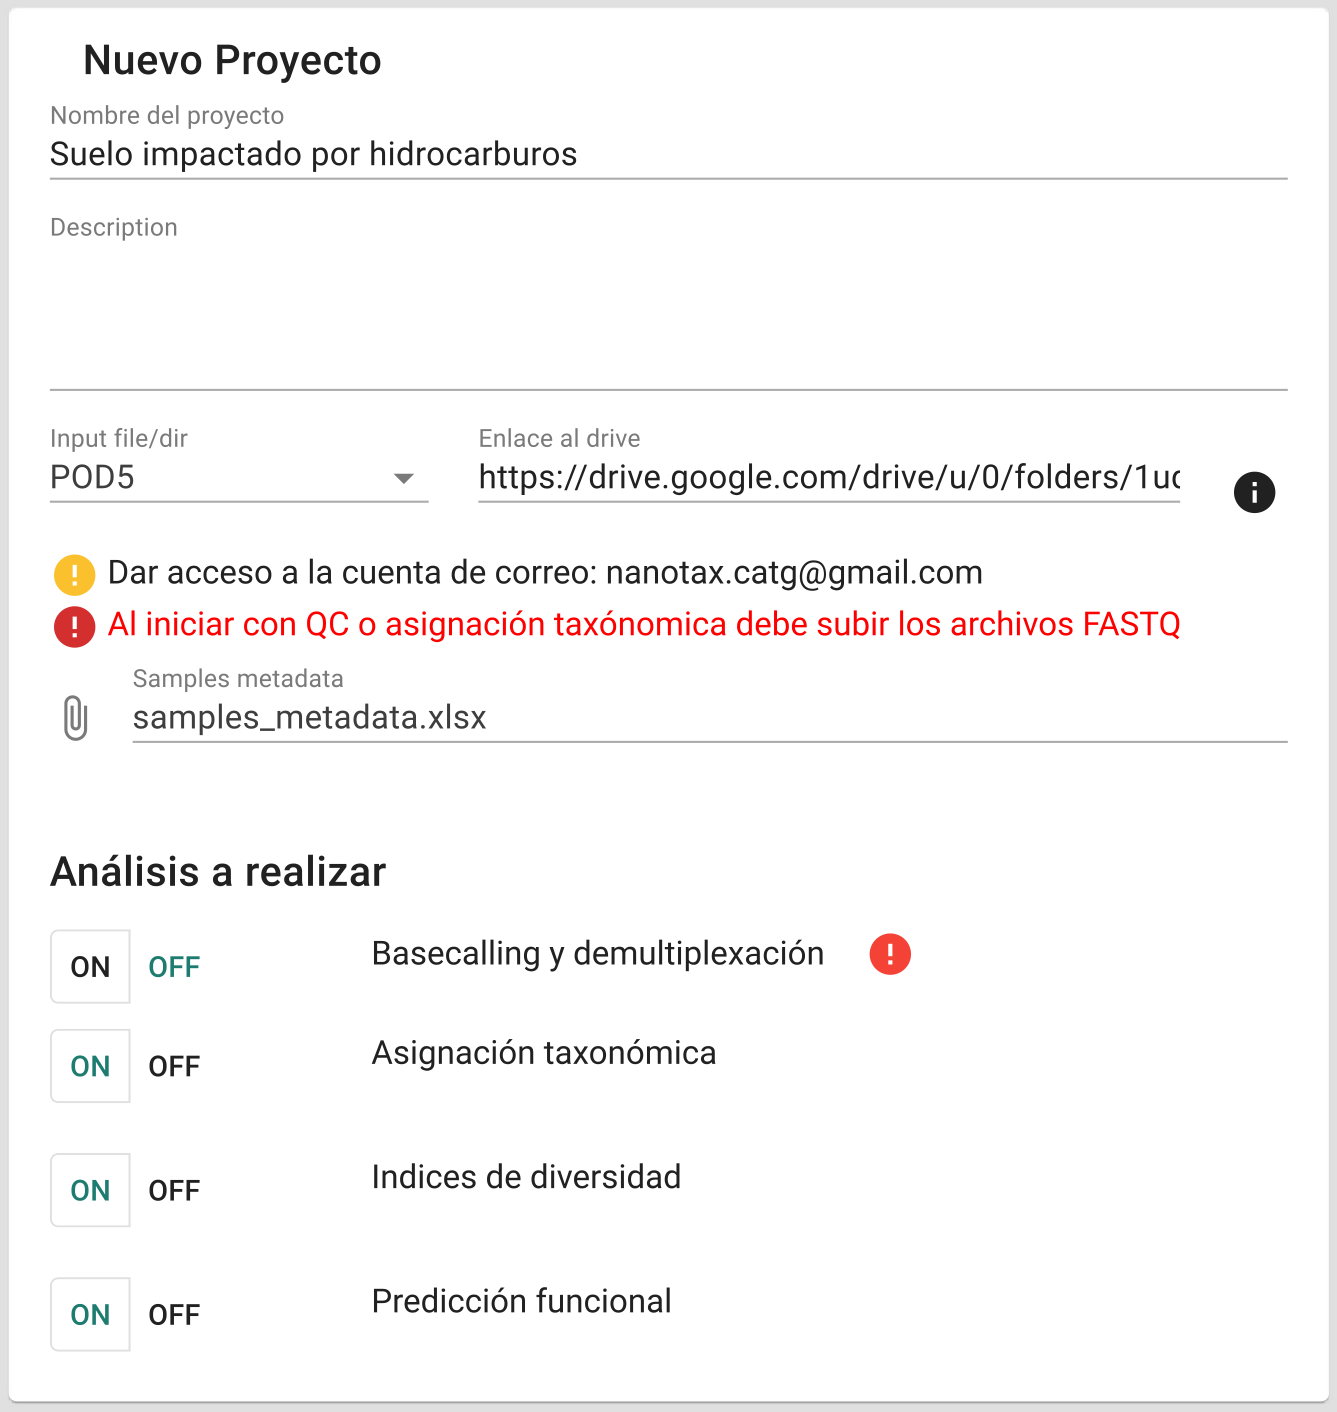
\includegraphics[width=\textwidth]{images/app/newAnalysis/fastq.png}
        \caption{Vista de nuevo análisis: Error al seleccionar el tipo del archivo}
        \label{fig:app-new-analysis-fastq-error}
    \end{subfigure}
    \caption{Vista de nuevo análisis: Error al seleccionar el tipo del archivo}
    \label{fig:app-new-analysis-type-file-error}
\end{figure}



\begin{figure}[H]
    \centering
    \begin{subfigure}[b]{0.45\textwidth}
        \centering
        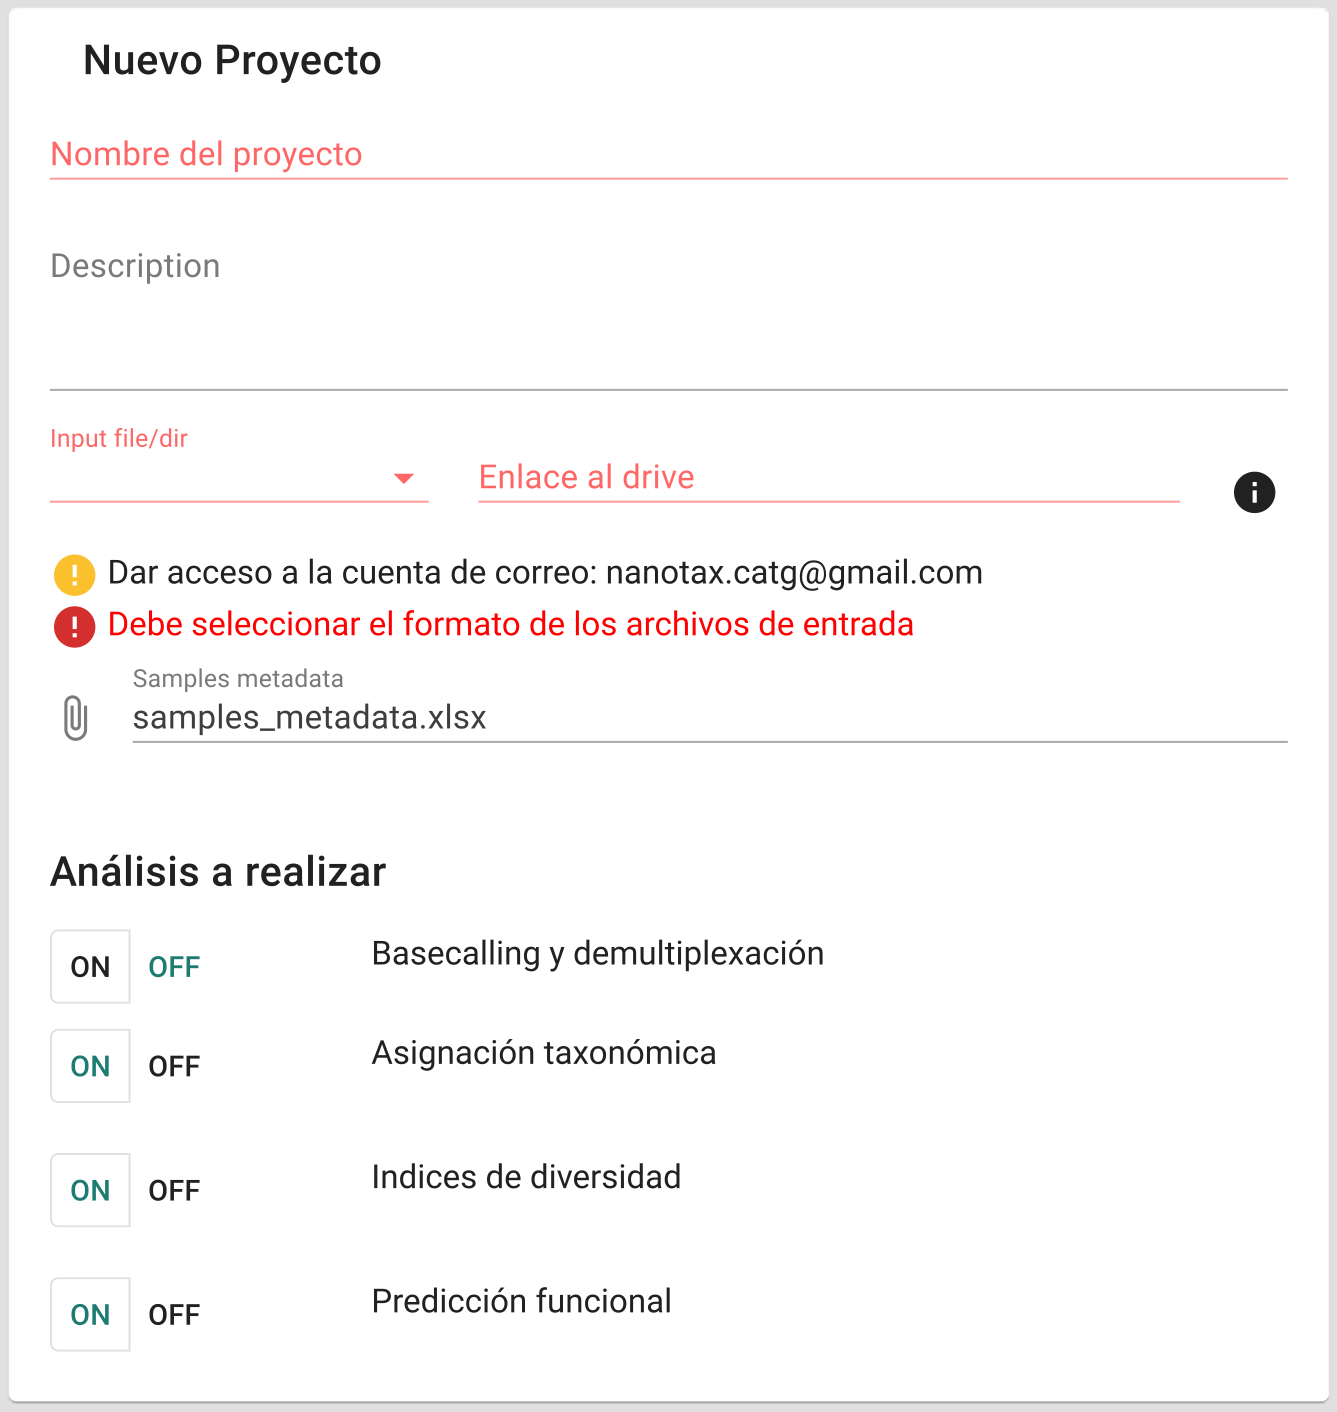
\includegraphics[width=\textwidth]{images/app/newAnalysis/errors1.png}
        \caption{Vista de nuevo análisis: Errores por falta de información}
        \label{fig:app-new-analysis-nodata-error}
    \end{subfigure}
    \hfill
    \begin{subfigure}[b]{0.45\textwidth}
        \centering
        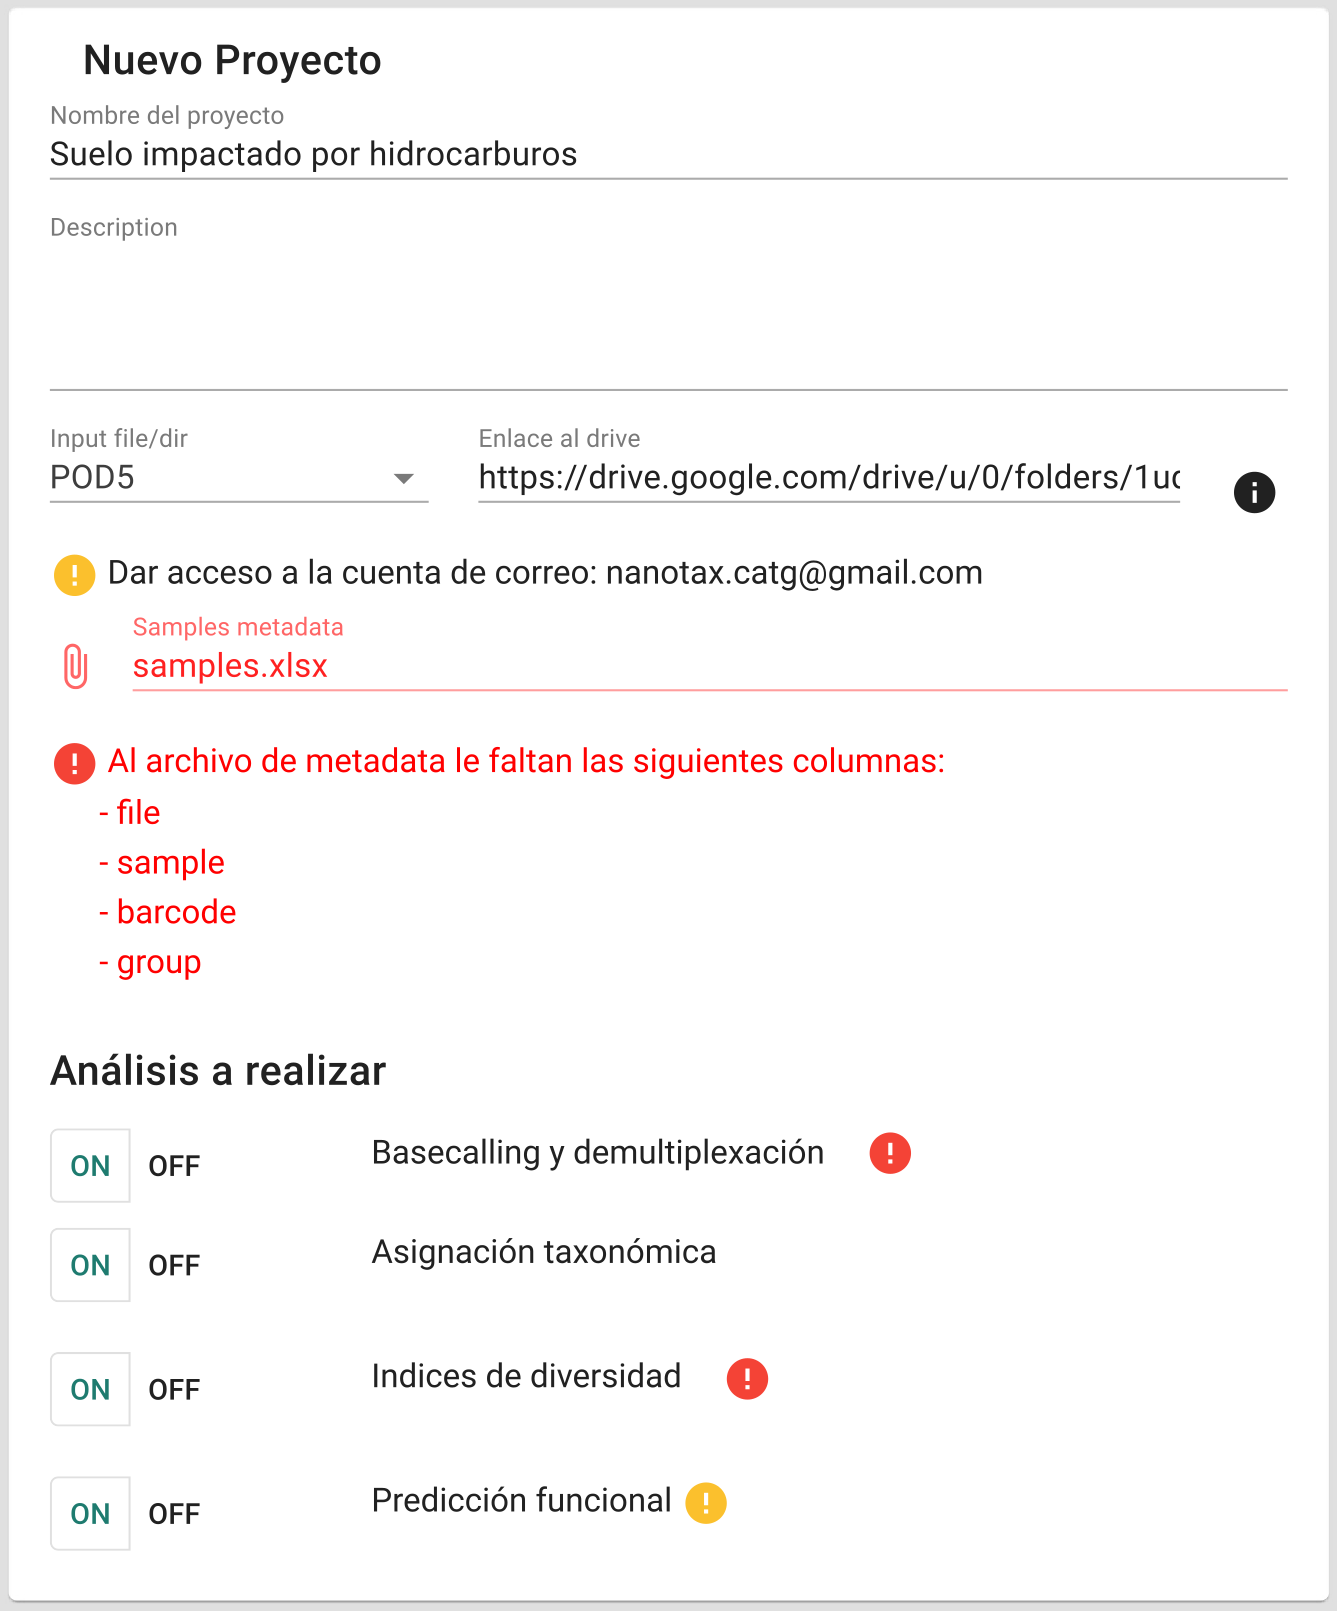
\includegraphics[width=\textwidth]{images/app/newAnalysis/metadata-error-1.png}
        \caption{Vista de nuevo análisis: Errores en el archivo de metadata}
        \label{fig:app-new-analysis-metadata-error}
    \end{subfigure}
    \caption{Vista de nuevo análisis: Errores }
    \label{fig:app-new-analysis-metadata-nodata-error}
\end{figure}









%%%%%%%%%%%%%%%%%%%%%%%%%%%%%%%%%%%%%%%%%%%%%%%%%%%%%%%%%%%%%%%%%%%%%%

\subsection{Resultados/Proyectos} \label{projects}
\hl{hacer}
Una vez que el usuario valida sus credenciales en la plataforma será redireccionado a la sección de Resultados. En esta sección se mostraran los proyectos que el usuario ha subido a la plataforma, estos proyectos pueden estar en ejecución, finalizados o finalizados con errores. 
Por cada proyecto se desplegará la información básica en una tarjeta:
\begin{itemize}
    \item Nombre del proyecto
    \item Descripción del proyecto
    \item Cantidad de muestras procesadas, descartadas y totales
    \item Estado del proyecto (upload\_data / running / failed / finish)
    \item En caso de que el proyecto haya finalizado el usuario podrá acceder a la sección especifica de resultados del proyecto mediante el botón de Ver resultados.
\end{itemize}



En la parte inferior del componente se encuentra el botón de Subir data, el cual al hacer click en el, ingresará la información a la base de datos y copiará los archivos a la plataforma de computo. Una vez que el usuario presionar el botón de subir data, la plataforma se encarga de verificar que se cuente con toda la información necesaria para correr el pipeline.
\subsection{Resultados de un proyecto en especifico}
Una vez que el pipeline haya finalizado su ejecución, la plataforma permitirá al usuario acceder a los resultados de cada proyecto leyendo los resultados desde la base de datos y desplegando la información en la sección de resultados de cada proyecto.
Esta sección cuenta con 5 subsecciones, cada una con información específica del análisis realizado. 
En caso de que al ingresar el proyecto el usuario no seleccione todos los análisis, solo se mostrarán las secciones indicadas por el usuario.

\subsubsection{Información básica de las muestras}
%Esta sección se mostrará siempre que el usuario empiece con archivos POD5 o FastQ, es decir, ya sea comenzando el análisis desde el basecalling o desde el control de calidad. \hl{Igual si es que solo se hace asignaicón taxonomica}.
\hl{Esta sección se desplegará siempre en la plataforma} y cuenta en el lado izquierdo con una tabla con información básica de las muestras y en el lado derecho un gráfico que representa la calidad y tamaño promedio de las lecturas.
La tabla esta compuesta por los siguientes elementos:
\begin{itemize}
    \item Nombre de la muestra: Nombre indicado en el archivo de metadata al ingresar el proyecto.
    \item \hl{Grupo}: Grupo asociado a la muestra en el archivo de metadata (en caso de ingresar grupo).
    \item Total de lecturas: Cantidad de lecturas previo a los filtros de calidad.
    \item Calidad promedio: Calidad promedio en formato phred \hl{antes/despues} de los filtros de calidad.
    \item Largo promedio: Largo promdio \hl{antes/despues} de los filtros de calidad
    \item Lecturas después de los filtros: Cantidad de lecturas luego de los filtros de calidad.
    \item Nota: Si la muestra fue descartada por no contar con la cantidad suficiente de lecturas se informará en esta columna.
\end{itemize}
En la parte inferior de la tabla hay una nota que indica la cantidad de lecturas que se consideraron para los análisis posteriores, este valor por defecto es \hl{100.000}, pudiendo ser modificado por el usuario en las opciones avanzadas al ingresar el proyecto.

En la parte derecha de la sección se puede visualizar un \hl{heatmap} donde en el eje X se encuentra el tamaño de las secuencias, y en el eje Y la calidad. 
El color indica la cantidad de lecturas que se encuentran en esa intersección, mientras más intenso el azul, más secuebcias tienen la calidad y tamaño indicado.
Para este grafico se consideraron todas las muestras con sus lecturas después de los filtros de calidad.

En la parte inferior del gráfico hay una nota que indica en que rangos de tamaño se encuentran la mayoria de las lecturas\hl{Muy generico?}. 
\begin{figure}[H]
    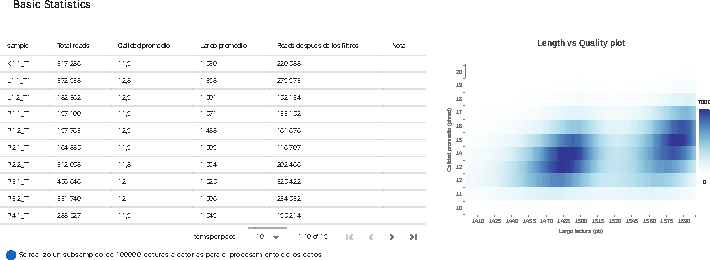
\includegraphics[width=1\linewidth]{images/app/results/basicStatistics.png}
    % \captionsetup{justification=raggedright, width=0.45\linewidth, singlelinecheck=off}

    % \captionsetup{width=0.45\linewidth}
    \caption{Estadisticas básicas (resultados)}
    \label{fig:app-results-basicStatistics}
\end{figure}

\subsection{Asignación taxonómica}
En la parte superior de esta sección se pueden visualizar pestañas que representan cada categoría taxonómica (especie, género, familia, orden, clase y filo), las cuales permiten ajustar la información presentada en esta  sección (gráfico de barras apiladas y tabla). Por defecto se presenta la información para la categoría de especie.

Debajo de las pestañas en el lado izquierdo hay un gráfico de barras apiladas que permite visualizar la abundancia de las taxonomías en cada muestra.
El usuario puede interactuar con el gráfico modificando la visualización a través de los botones que se encuentran en la parte inferior, pudiendo visualizar la información en porcentaje o en cantidad de lecturas, como también pudiendo modificar el porcentaje mínimo para crear la categoria \textit{Otros}.
En caso de que el usuario hubiera ingresado información de grupos asociados a las muestras, se podrá visualizar un nuevo grupo de botones que permite al usuario visualizar la información de las taxonomías por grupo o por muestra.
La leyenda del gráfico de barras apiladas presenta solo las 10 taxonomías con mayor abundancia. 
Por defecto, todas aquellas taxonomías que tienen un porcentaje menor a un 1\%  son agrupadas en una nueva taxonomia llamada \textit{Otros}.



En el lado derecho, hay una tabla que permite visualizar el detalle de la información presentada en el gráfico. Se puede visualizar además un campo de texto que permite al usuario buscar una taxonomía en especifico y visualizar su abundancia o cantidad de lecturas en todas las muestras.


Ambos componentes, la tabla y el gráfico de barras apiladas se ajustan automáticamente para presentar la información requerida por el usuario, es decir, cada vez que el usuario selecciona una nueva categoría taxonómica en las pestañas, se vuelve a generar la información proporcionando una visualización clara y detallada de los datos.


\begin{figure}[H]
    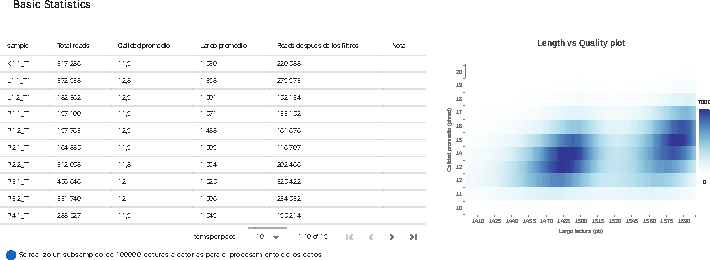
\includegraphics[width=0.6\linewidth, heigth=1]{images/app/results/basicStatistics.png}
    % \captionsetup{justification=raggedright, width=0.45\linewidth, singlelinecheck=off}

    % \captionsetup{width=0.45\linewidth}
    \caption{Estadisticas básicas (resultados)}
    \label{fig:app-results-taxonomicAssig-sample-nreads}
\end{figure}

\begin{figure}[H]
    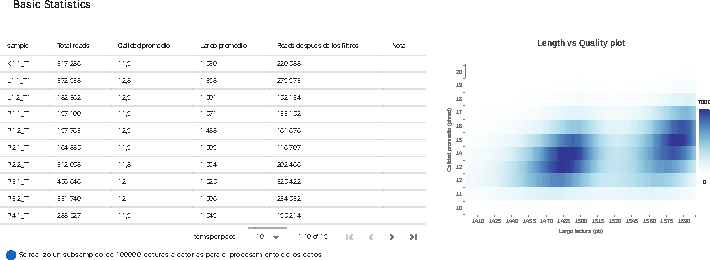
\includegraphics[width=1\linewidth]{images/app/results/basicStatistics.png}
    % \captionsetup{justification=raggedright, width=0.45\linewidth, singlelinecheck=off}

    % \captionsetup{width=0.45\linewidth}
    \caption{Estadisticas básicas (resultados)}
    \label{fig:app-results-taxonomicAssig-sample-perc}
\end{figure}

\begin{figure}[H]
    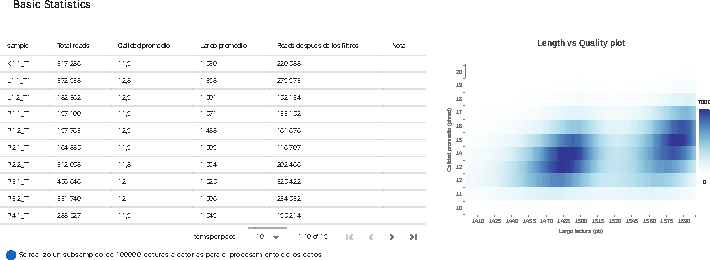
\includegraphics[width=1\linewidth]{images/app/results/basicStatistics.png}
    % \captionsetup{justification=raggedright, width=0.45\linewidth, singlelinecheck=off}

    % \captionsetup{width=0.45\linewidth}
    \caption{Estadisticas básicas (resultados)}
    \label{fig:app-results-taxonomicAssig-group-nreads}
\end{figure}

\begin{figure}[H]
    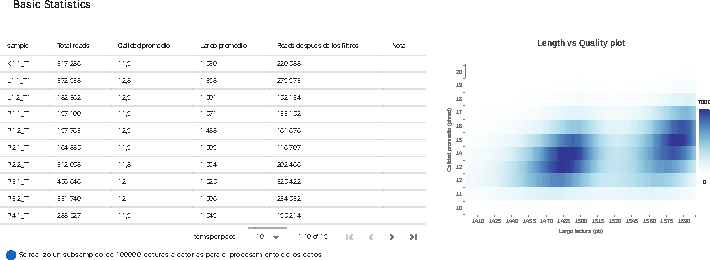
\includegraphics[width=1\linewidth]{images/app/results/basicStatistics.png}
    % \captionsetup{justification=raggedright, width=0.45\linewidth, singlelinecheck=off}

    % \captionsetup{width=0.45\linewidth}
    \caption{Estadisticas básicas (resultados)}
    \label{fig:app-results-taxonomicAssig-group-perc}
\end{figure}
\subsection{Similitud entre las muestras}
\hl{la info es la suma de todo?}


Esta sección representa las taxonomías compartidas por las muestras mediante un gráfico circular de anillos jerarquicos. 
Cada nivel del gráfico representa una categoría taxonómica, siendo la más interna especie, y la más externa filo.
Mientras más grande el diamentro del anillo en el gráfico, mayor es la presencia de esa taxonomía en las muestras.

En esta sección se puede presentar un solo gráfico de las taxonomías compartidas entre todas las muestras, y en el caso de que el usuario haya ingresado grupos, se desplegaran además los gráficos por cada grupo.
En la parte inferior del gráfico, al lado derecho de la leyenda se puede visualizar un icono, el cual al posicionarse sobre el, va a mostrar las muestras utilizadas para generar el gráfico.

\begin{figure}[H]
    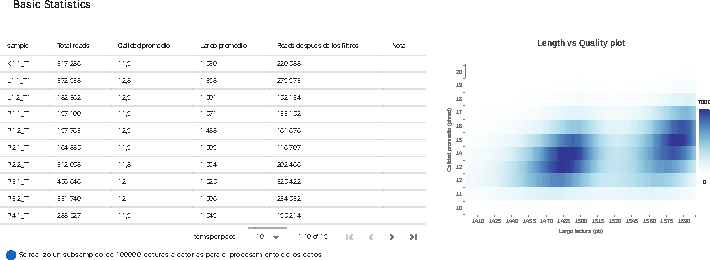
\includegraphics[width=1\linewidth]{images/app/results/basicStatistics.png}
    % \captionsetup{justification=raggedright, width=0.45\linewidth, singlelinecheck=off}

    % \captionsetup{width=0.45\linewidth}
    \caption{Gráfico de similitud  (resultados)}
    \label{fig:app-results-core}
\end{figure}

\begin{figure}[H]
    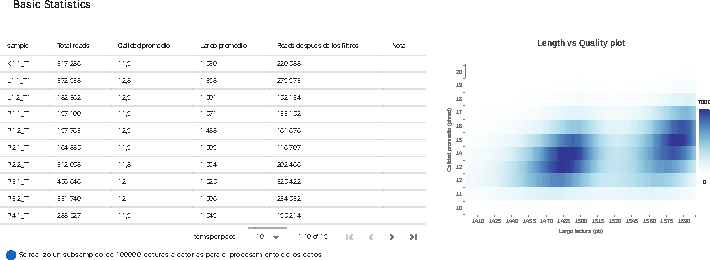
\includegraphics[width=1\linewidth]{images/app/results/basicStatistics.png}
    % \captionsetup{justification=raggedright, width=0.45\linewidth, singlelinecheck=off}

    % \captionsetup{width=0.45\linewidth}
    \caption{Gráfico de similitud: Tooltip asociado a las muestras (resultados)}
    \label{fig:app-results-core-tooltip}
\end{figure}

\hl{En caso de que un grupo no tenga taxonomías compartidas entre si, se desplegará un mensaje indicando esto.}
\subsubsection{Indices de diversidad}
\hl{hacer}

En caso de que el usuario hubiera ingresado grupos al inicio del proyecto, se podrá visualizar tres gráficos boxplot, uno por cada indice de diversidad (Shannon, Simpson y Chao2). En caso de que el usuario no haya ingresado grupos, esta sección no se desplegará en la plataforma.


\subsubsection{Predicción funcional}
Al igual que en la sección de asignación taxonómica, en la parte superior se pueden visualizar tres pestañas \textit{EC, KO y Pathways} que representan cada categoría funcional. Por defecto se presenta la información para la categoría de \textit{Pathways}.

En la parte inferior izquierda se puede visualizar una tabla con la información de la predicción funcional obtenida mediante PICRUSt2 (EC, KO y Pathways) para cada muestra. 
En la parte superior de la tabla se puede visualizar un campo de texto de búsqueda con el cual el usuario puede filtrar la información de la tabla.

En el lado derecho de la sección, en caso de que el usuario hubiera ingresado grupos, se puede ver un gráfico de barras horizontales que muestra los pathways con diferencias significativas entre los grupos (información obtenida mediante \hl{Lefse}). 
En caso de que no se haya ingresado información de grupos, solo se desplegará la tabla.

Al igual que en la sección de asignación taxonómica el usuario puede interactuar con las pestañas modificando el contenido de las tablas mediante la selección de las pestañas.


\begin{figure}[H]
    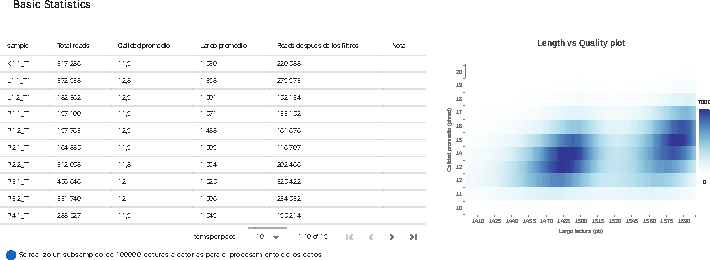
\includegraphics[width=1\linewidth]{images/app/results/basicStatistics.png}
    % \captionsetup{justification=raggedright, width=0.45\linewidth, singlelinecheck=off}

    % \captionsetup{width=0.45\linewidth}
    \caption{Gráfico de similitud: Tooltip asociado a las muestras (resultados)}
    \label{fig:app-results-functional}
\end{figure}
\subsubsection{Descarga de los resultados}
En la parte superior derecha de la sección de resultados, se encuentra un botón con el texto \textit{Download data}. 
Al hacer click en este botón se descargará un archivo comprimido con toda los resultados generados por el pipeline.
A continuación se detallan los archivos:
\begin{itemize}
    \item CSV de asignación taxonomica por muestra y por grupo (en caso de ingresarse), y por porcentaje y cantidad de lecturas
    \item CSV de predicción funcional (EC, KO y pathways), en caso dehaber seleccionado predicción funcional dentro de los análisis.
    \item CSV con los valores del cálculo de los indices de diversidad
    \item \hl{PDF con los gráficos de barras apiladas, Sunburst y boxplot}
    \item \hl{Archivo de texto con la información del pipeline (versión, parámetros, etc)}
\end{itemize}

\begin{figure}[H]
    \includegraphics[width=1\linewidth]{images/app/results/downloadbutton.png}
    % \captionsetup{justification=raggedright, width=0.45\linewidth, singlelinecheck=off}

    % \captionsetup{width=0.45\linewidth}
    \caption{Botón de descarga de resultados(resultados)}
    \label{fig:app-results-download}
\end{figure}
\subsection{Documentación}
En esta sección se despliega la documentación del pipeline, la cual cuenta con la información de los módulos, parámetros y herramientas utilizadas en el pipeline. La documentación se encuentra dividida por cada módulo, donde se muestra la versión de la herramienta utilizada y los parámetros por defecto y modificables por el usuario.
\subsubsection{Basecalling y demultiplexación}
\subsubsection{Control de calidad}
\subsubsection{Asignación taxonómica}
\subsubsection{Predicción funcional}
\subsubsection{Indices de diversidad}

